% --- thesis/main.tex ---
\documentclass[11pt,a4paper,oneside]{book}

% --- thesis/preamble.tex ---
\usepackage{iftex}
\ifPDFTeX
    \usepackage[utf8]{inputenc}
    \usepackage[T1]{fontenc}
\fi
\usepackage{fontspec}
\usepackage{newtxtext}
\usepackage{newtxmath}
\newfontfamily\coverfont[
    Path=/System/Library/Fonts/Supplemental/,
    UprightFont={Times New Roman.ttf},
    BoldFont={Times New Roman Bold.ttf},
    ItalicFont={Times New Roman Italic.ttf},
    BoldItalicFont={Times New Roman Bold Italic.ttf}
]{Times New Roman}
\usepackage{microtype}
\usepackage{geometry}
\geometry{a4paper, left=30mm, right=25mm, top=30mm, bottom=30mm}

\usepackage{fancyhdr}
\setlength{\headheight}{14.5pt}
\pagestyle{fancy}
\fancyhf{}
\fancyhead[L]{\MakeUppercase{\leftmark}}
\fancyfoot[C]{\thepage}
\renewcommand{\headrulewidth}{0.4pt}

\usepackage{graphicx}
\usepackage{amsmath}
\let\Bbbk\undefined
\usepackage{amssymb,amsfonts}
\usepackage{algorithmic}
\usepackage{algorithm}
\usepackage{xcolor}
\usepackage{booktabs}
\usepackage{multirow}
\usepackage{array}
\usepackage{tabularx}
\usepackage{enumitem}
\usepackage{cite}
\usepackage{setspace}
\usepackage{titlesec}
\usepackage{caption}
\usepackage{subcaption}
\PassOptionsToPackage{hidelinks}{hyperref}

% TikZ
\usepackage{tikz}
\usetikzlibrary{calc,positioning,shapes.geometric,arrows.meta,3d,shadows}

% Hyperref
\usepackage{hyperref}
\usepackage{bookmark}
\hypersetup{pdftitle={Hardware-Software Co-Design for Scalable Long-Context Large Language Models}, pdfauthor={Kaichen Li}}
\captionsetup{font=small, labelfont=bf}
\widowpenalty=10000
\clubpenalty=10000
\emergencystretch=2em
\setlist{itemsep=0.25em, topsep=0.35em}

% Line spacing for thesis
\setstretch{1.5}


\begin{document}
\pagenumbering{gobble}

\begin{titlepage}
\thispagestyle{empty}
\begingroup
\coverfont
\singlespacing
\setlength{\parindent}{0pt}
\begin{center}
    \vspace*{9mm}

    {\fontsize{13}{16}\selectfont Research Report\par}

    \vspace{16mm}

    {\fontsize{22}{28}\selectfont
    \begin{minipage}{0.90\textwidth}
        \centering\coverfont\bfseries
        Hardware-Software Co-Design for Scalable Long-Context Large Language Models
    \end{minipage}\par}

    \vspace{7mm}

    {\fontsize{16}{20}\selectfont Integer PIM and CXL Pooling\par}

    \vspace{21mm}

    {\fontsize{13}{16}\selectfont June 2026\par}

    \vspace{15mm}

    {\fontsize{13}{16}\selectfont Major of Computer Science and Technology\par}
    \vspace{3mm}
    {\fontsize{13}{16}\selectfont Graduate School of Computer Engineering Youngsan University\par}

    \vspace{16mm}

    {\fontsize{13}{16}\selectfont \textbf{Kaichen Li}\par}

    \vspace{30mm}

    {\fontsize{13}{16}\selectfont Supervised by \textbf{Gilja So}\par}

    \vspace{27mm}

    {\fontsize{13}{16}\selectfont Graduate School of Computer Engineering\par}
    \vspace{4mm}
    {\fontsize{13}{16}\selectfont Youngsan University\par}
\end{center}
\endgroup
\end{titlepage}

\cleardoublepage
\frontmatter

\chapter*{Abstract}
\addcontentsline{toc}{chapter}{Abstract}
Long-context Large Language Model (LLM) serving turns the Key-Value (KV) cache from an implementation detail into a memory-system bottleneck. In the 128K-token configuration evaluated here, one 7B-class grouped-query request already reserves several gigabytes for stored keys and values. A larger memory tier can hold that state, but capacity alone does not decide decode speed. If each new token still pulls large regions of the old cache through a host-centered Compute Express Link (CXL) path, the expanded tier becomes a new source of shared-link traffic.

The report is organized around two artifacts rather than one monolithic accelerator. In \textbf{LKC-CXL-PIM}, the historical K/V pages stay in a CXL-attached HBM stack. A decode request reaches the endpoint as a compact descriptor containing the query vector, page range, head id, and scale metadata; the endpoint then walks its local cache and returns the weighted attention result. The fixed-point Integer Non-Linear Unit (iNLU) keeps the softmax exponential on the integer path, and the overflow route is used only for activations that would be damaged by the dense INT8 lane. \textbf{DisaggKV} carries the same idea into a memory pool: shared prefix pages are kept reusable, private continuation pages are spread across endpoints, and the only softmax values exchanged globally are the maximum and exponential sum.

I keep the measurement evidence split for auditability. Modified Ramulator 2.0 traces provide the HBM/PIM timing, a Python CXL-fabric event model supplies multi-node queueing behavior, and synthesis-derived proxy reports bound the iNLU cost. With a 128K-token single-endpoint trace, LKC-CXL-PIM lowers read latency from 77.90 million cycles to 0.80 million cycles and reduces normalized logic-die area from 1.00 to 0.83. In the distributed runs, DisaggKV stays within a 50\,ms tail-latency target until roughly 2.9K requests/s, cuts host-facing traffic by 92.2\% per 1M decoded tokens, and reaches a 95th-percentile recovery latency of 416\,ms under the injected-fault model.

\tableofcontents
\listoffigures
\listoftables

\mainmatter

\chapter{Introduction}
\label{ch:introduction}

\section{The Rise of Long-Context Large Language Models}
Large Language Models (LLMs) are no longer used only for short prompt completion. Current serving workloads often keep a document set, a code base, or a long dialogue history inside the same session. Model families such as LLaMA and Qwen now advertise context windows that would have looked unusual only a few years ago~\cite{llm_context, ring_attention}. The hardware consequence is easy to miss: a token admitted early in the session becomes part of the state that later tokens must revisit.

The checked traces pushed me away from treating this as only a matrix-throughput problem. For 2K and 8K contexts, the dense kernels are still visible enough that a faster arithmetic block matters. By 64K and 128K tokens, however, the repeated walk over old cache lines is the part that dominates my reading of the run. The serving system has to keep the KV cache resident, spill it when local HBM is short, and touch earlier tokens again for every decoded token. If that cache is sharded, the old state also has to agree across devices. That is why the later experiments focus on stored history and host-facing movement instead of only on a larger matrix unit.

\section{The Generative Memory Wall}
The serving path has two phases with very different memory behavior. In prefill, prompt tokens are processed together, and the matrix engines can exploit parallelism across the input sequence. Decode is the awkward phase for memory systems. Only one token is produced at a time, but that token still needs the \textit{Key-Value (KV) cache}: the query for the new token is scored against the keys and values saved from the entire prior history~\cite{vllm}.

The result is a state object whose size is tied directly to the usable context length. A 7B-class model with a $128{,}000$-token context can require several gigabytes of KV-cache storage for one request before batching or concurrent sessions are considered~\cite{vllm}. At that point, the problem is not simply how many multiply-accumulates the accelerator can issue; it is whether the memory hierarchy can hold the history and feed it back to the decode loop quickly enough.

Off-package memory expansion, including Compute Express Link (CXL) memory tiers, is a natural response when the cache no longer fits comfortably in local HBM~\cite{cxl_standard}. The catch is that capacity and movement are separate problems. A remote tier can hold the cache, but a conventional data path still pays to bring large portions of that cache back toward the host or accelerator during decode.

\section{Challenges in Existing Infrastructures}

\subsection{CXL and the Bandwidth Bottleneck}
Compute Express Link maps remote memory devices into the host's address space and makes pooled capacity easier to expose to software~\cite{cxl_pond}. For KV-cache serving, that abstraction is helpful but incomplete. The Root Complex and switch ports can become the busy part of the system, especially when the remote memory device is used as a passive store. In that host-aggregated path, the host or accelerator fetches KV tensors across the interconnect, performs attention-side work elsewhere, and repeats the transfer on the next token. With long contexts and many active requests, the repeated movement consumes shared bandwidth and creates queueing delay at the CXL switch ports~\cite{distserve}.

\subsection{Processing-in-Memory and Format Mismatches}
Processing-in-Memory (PIM) attacks the movement problem from the opposite direction: let memory-side logic consume the data before it leaves the package~\cite{samsung_pim}. For this thesis, the awkward part is numeric rather than conceptual. Serving stacks often keep KV caches in INT8 or INT4 forms to stretch effective capacity~\cite{llm_outliers, gptq}, while many PIM datapaths are designed around floating-point nonlinear units. If an endpoint first dequantizes KV data, then runs floating-point softmax, then reformats the result, the design spends too much of its locality advantage on conversion.

\section{Research Motivation and Objectives}
The design work in this report starts from a specific reading of the traces: for long-context decode, the limiting object is the KV cache, not the multiply-accumulate array. The useful question is where the cache is placed, how often it crosses an off-package link, and whether the nonlinear part of attention can run in the same compact numeric format used for storage.

Two design rules came out of this reading. First, a CXL endpoint should consume the KV cache in the format used by the serving stack; otherwise conversion becomes a second memory-side bottleneck. Second, a distributed memory pool should move only the softmax bookkeeping values that truly have to be global. The old K/V history is the expensive object, so a path that pulls it back to the host remains the baseline to beat.

\section{Claim Boundary}
I draw the boundary around the KV cache rather than around the whole Transformer. Model weights, dense matrix kernels, and the rest of the decoder stack remain on the accelerator side. The object allowed to move is the long-lived KV state, either into one CXL-attached HBM tier or across several CXL memory endpoints. This choice keeps the proposal independent of sparsity, attention approximation, prompt compression, and KV-cache compression. The narrower question is the one I can test with the artifact: if the cache has to remain available for future tokens anyway, how much host-facing traffic disappears when attention-side traversal runs beside that cache?

The evidence is separated for the same reason. There is no fabricated chip behind this report, so I do not present the result as one end-to-end silicon measurement. Single-endpoint timing comes from modified Ramulator runs; cluster behavior comes from the CXL-fabric event model; iNLU area and power come from synthesis proxy reports. The split is not pretty, but it keeps the assumptions visible. DRAM timing, switch queueing, and nonlinear datapath cost can be inspected separately instead of being hidden inside one speedup number.

\section{Thesis Contributions}
For the single-endpoint artifact, I built the datapath around one deliberately narrow job: let the CXL endpoint perform the attention work that repeatedly touches stored KV state, while the host and accelerator keep the rest of the generation pipeline. The endpoint receives a query descriptor, walks the HBM-resident K/V pages, and returns a compact attention result. The iNLU replaces the FP16 exponential path with range reduction, a quadratic fixed-point approximation, and shift scaling. The outlier front-end keeps ordinary activations on the dense INT8 lane and sends rare large values to a small INT32 buffer. In the 128K-token evaluation, this organization lowers read latency by more than 98.9\% and reduces normalized logic-die area by 17\% relative to the floating-point baseline.

DisaggKV is the pool-scale artifact. It starts from the case where a request's KV state is too large, or too shared, to treat as one endpoint's private region. Reused prefix pages are kept stable so later sessions can attach to them, while private continuation pages are spread enough to avoid turning one endpoint into the sink for a request's history. The reduction protocol then moves only two global softmax values across shards. In the modeled multi-tenant run, combined interconnect traffic falls by about 84\%, host-facing traffic by more than 90\%, the 50\,ms tail target holds until roughly 2.9K requests/s, and injected-fault recovery remains below one second.

\section{Thesis Organization}
The remaining chapters follow the order in which the design was built. Chapter~\ref{ch:background} records the attention, CXL, queueing, and PIM concepts used later. Chapter~\ref{ch:motivation} shows why the checked traces point to both capacity pressure and repeated movement. Chapters~\ref{ch:inlu_architecture} and~\ref{ch:disaggkv_system} describe the two artifacts: first one CXL-attached HBM endpoint, then a distributed CXL memory pool. Chapter~\ref{ch:methodology} explains the simulation inputs and provenance, Chapter~\ref{ch:evaluation} reports the measured trends, Chapter~\ref{ch:related_work} positions the work against nearby systems, and Chapter~\ref{ch:conclusion} closes with the remaining limitations.

\chapter{Background}
\label{ch:background}

This chapter gives only the background needed to understand the design choices later in the report. The thread running through the chapter is the same one that appeared in the traces: the KV cache grows linearly, but the penalty for that growth is paid repeatedly during decode. CXL helps with capacity, queueing explains why host-facing links become painful under load, and quantization explains why a near-memory design cannot simply attach a floating-point softmax block to an integer cache.

\section{LLM Inference Dynamics and the KV Profile}

Autoregressive Transformer inference repeatedly evaluates self-attention over an expanding history. During decode, the current query vector $\mathbf{Q}$ must be compared against the stored key and value tensors accumulated from previous tokens~\cite{flashattn}. The standard formulation is:
\begin{equation}
\label{eq:attn}
\text{Attention}(\mathbf{Q}, \mathbf{K}, \mathbf{V}) = \text{Softmax}\left( \frac{\mathbf{Q} \mathbf{K}^T}{\sqrt{d}} \right) \mathbf{V}
\end{equation}

For a batch size $B$, sequence length $L$, number of attention heads $H$, and head dimension $d$, the storage requirement of an FP16 KV cache is:
\begin{equation}
    \text{Size}_{KV} = 2 \times B \times L \times H \times d \times (\text{2 bytes})
\end{equation}
Because the KV cache scales linearly with $L$, the stored state becomes the part of decode that is hardest to ignore. Prior systems work has shown the same tendency from a different angle: as sequences lengthen, more time and energy are spent managing the cache rather than only executing dense arithmetic~\cite{infinigen}.

\section{Compute Express Link (CXL) and Tiered Memory}

HBM offers very high bandwidth but limited capacity per accelerator package. As model size, batch size, and context length continue to grow, that fixed on-package capacity becomes increasingly restrictive. Compute Express Link (CXL) addresses this problem by enabling memory expansion and pooling over PCIe-based links while preserving a load/store programming model~\cite{cxl_standard}.

Type-3 CXL devices act as memory expanders that can be mapped directly into the host memory space without requiring an RDMA-style communication stack~\cite{direct_cxl}. That programming model is convenient for long-context serving because the cache can spill into a larger tier without rewriting the application around explicit messages. The cost is the gap between local HBM and a fabric-attached device. HBM access is measured in tens of nanoseconds and provides aggregate bandwidth on the order of TB/s, whereas a CXL path provides lower bandwidth and higher traversal latency~\cite{tpp}. Moving the KV cache from HBM to CXL therefore fixes one problem while making another one more visible.

\section{Queueing Theory and the Host-Aggregated Wall}

In current host-aggregated CXL deployments, remote accesses are still routed through the Root Complex. When many endpoints serve long-context decode requests concurrently, the host-facing links and switch ports become shared queueing resources. A useful approximation is the M/D/1 queue:
\begin{equation}
\label{eq:queue}
W_q = \frac{\rho}{2\mu(1 - \rho)} \quad \text{where} \quad \rho = \frac{\lambda}{\mu}
\end{equation}
Here, $\lambda$ is the aggregate arrival rate and $\mu$ is the service rate of the link or switch port~\cite{kleinrock}. In a long-context decode workload, the arrival term should be read as repeated fetch traffic for large KV-cache regions. Once utilization $\rho$ moves close to one, small increases in request rate produce a sharp increase in waiting time.

This is the point where a capacity solution becomes a traffic problem. If decode continues to pull dense KV tensors toward the host, a larger memory pool only gives the system more remote state to fetch. Reducing $\lambda$ in this setting requires a dataflow change, not only a larger addressable memory space.

\section{Processing-in-Memory and Model Quantization}

Processing-in-Memory places simple arithmetic units close to the memory arrays so that a larger fraction of the data path remains on the memory device rather than crossing the package boundary~\cite{pim_survey}. For attention workloads, this is attractive because the stored keys and values can be consumed where they reside.

\begin{sloppypar}
The complication is that the software stack and the memory-side logic often optimize for different numeric formats. Quantization methods such as SmoothQuant and GPTQ shrink model state and activations into low-precision integer representations~\cite{llm_smoothquant, gptq}. Many PIM proposals, including commercial HBM-PIM examples, keep floating-point datapaths because they target a broader mix of kernels~\cite{samsung_pim}. A KV cache that is stored compactly may therefore have to be expanded before the nonlinear attention stage can run near memory.
\end{sloppypar}

If quantized KV-cache data must be repeatedly up-converted to floating point inside the memory logic, the endpoint pays conversion cost before it earns the benefit of locality. The single-node design in this thesis therefore uses an integer-oriented nonlinear path and treats floating-point softmax as the baseline to beat, not as the default assumption for a PIM endpoint.

\chapter{Motivation: The Long-Context Memory Wall}
\label{ch:motivation}

The motivation in this chapter comes from the checked-in traces rather than from a generic claim that ``memory matters.'' In the short-context runs, dense compute is still visible enough that a faster matrix engine would help. In the long-context runs, the historical KV reads become the dominant term, and the useful decode rate is set by how quickly the memory system can revisit old tokens. I use that change in the trace profile to derive the requirements used in the two design chapters.

\section{The KV Cache Capacity and Bandwidth Crisis}

During decode, every new token consults the KV entries produced by prefill and by earlier decode iterations. The storage footprint grows one token at a time, while the read pressure is paid repeatedly at generation time. That asymmetry is what makes the cache more than a capacity bookkeeping problem.

\begin{figure}[htbp]
\centering
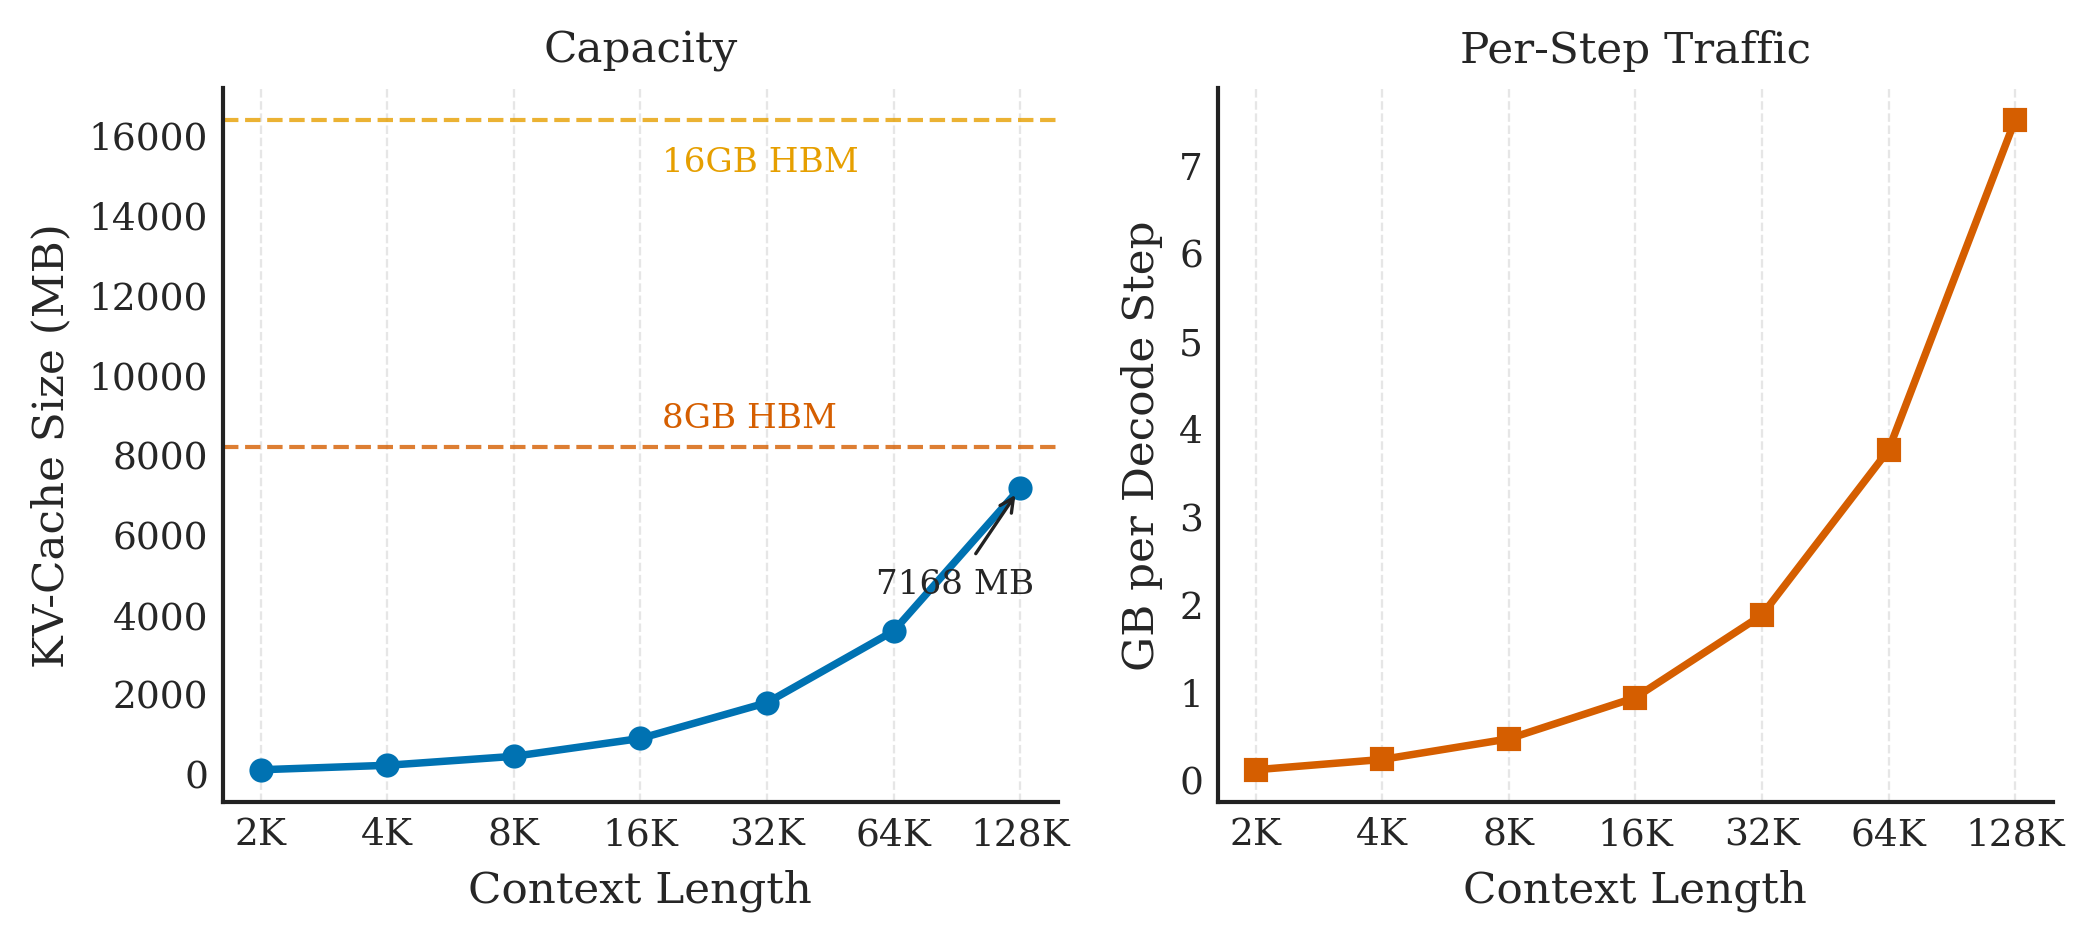
\includegraphics[width=\textwidth]{../paper_assets/figures/fig3_kv_cache_scaling.png}
\caption[KV-cache scaling with context length]{KV-cache processing scale factor as the sequence length approaches long-context settings without out-of-memory failures.}
\label{fig:scaling}
\end{figure}

Figure~\ref{fig:scaling} uses a Qwen2.5-7B-style configuration to show the scale of the state. With 28 layers, four grouped-query KV heads, 128 dimensions per head, and FP16 storage, one $128{,}000$-token request requires more than 7\,GB of KV-cache space~\cite{vllm}. That is already a large allocation for one user; under batching or multi-tenant serving, the same linear term quickly consumes the memory budget that would otherwise hold additional requests.

The same trend can be written as a simple per-token footprint. For the evaluated grouped-query configuration, each token contributes:
\begin{equation}
2 \times 28 \times 4 \times 128 \times 2 = 57{,}344 \ \text{bytes}
\end{equation}
where the leading factor of two accounts for keys and values. Table~\ref{tab:kv_footprint} expands this value across the context lengths used in the experiments. The table is useful because it separates capacity pressure from bandwidth pressure: the memory system must reserve the footprint once, but it must revisit the stored history during every decode step.

\begin{table}[htbp]
\centering
\caption[KV-cache footprint across context lengths]{Bytes reserved by one request in the Qwen2.5-7B-style trace; values follow from the grouped-query layout above.}
\label{tab:kv_footprint}
\begin{tabular}{lrr}
\toprule
\textbf{Context Length} & \textbf{Bytes per Request} & \textbf{Approx. Size} \\
\midrule
2K   & 117,440,512   & 112 MiB \\
8K   & 469,762,048   & 448 MiB \\
32K  & 1,879,048,192 & 1.75 GiB \\
64K  & 3,758,096,384 & 3.50 GiB \\
128K & 7,340,032,000 & 6.84 GiB \\
\bottomrule
\end{tabular}
\end{table}

CXL can provide the required capacity, but the traffic requirement remains severe. A decode stream that emits 20 tokens/s and repeatedly revisits multi-gigabyte historical state can quickly approach the practical bandwidth of a PCIe/CXL link~\cite{direct_cxl}. This is why the later designs treat long-context serving as both a placement problem and a movement problem.

\section{Latency Profiling}

The per-token profile is divided into three terms. The first term is model arithmetic on weights and the current hidden state. The second is format work, including unpacking or conversion when compressed integer state is consumed by a higher-precision compute path. The third is historical KV access, which covers movement and memory service time for keys and values generated by earlier tokens.

\begin{figure}[htbp]
\centering
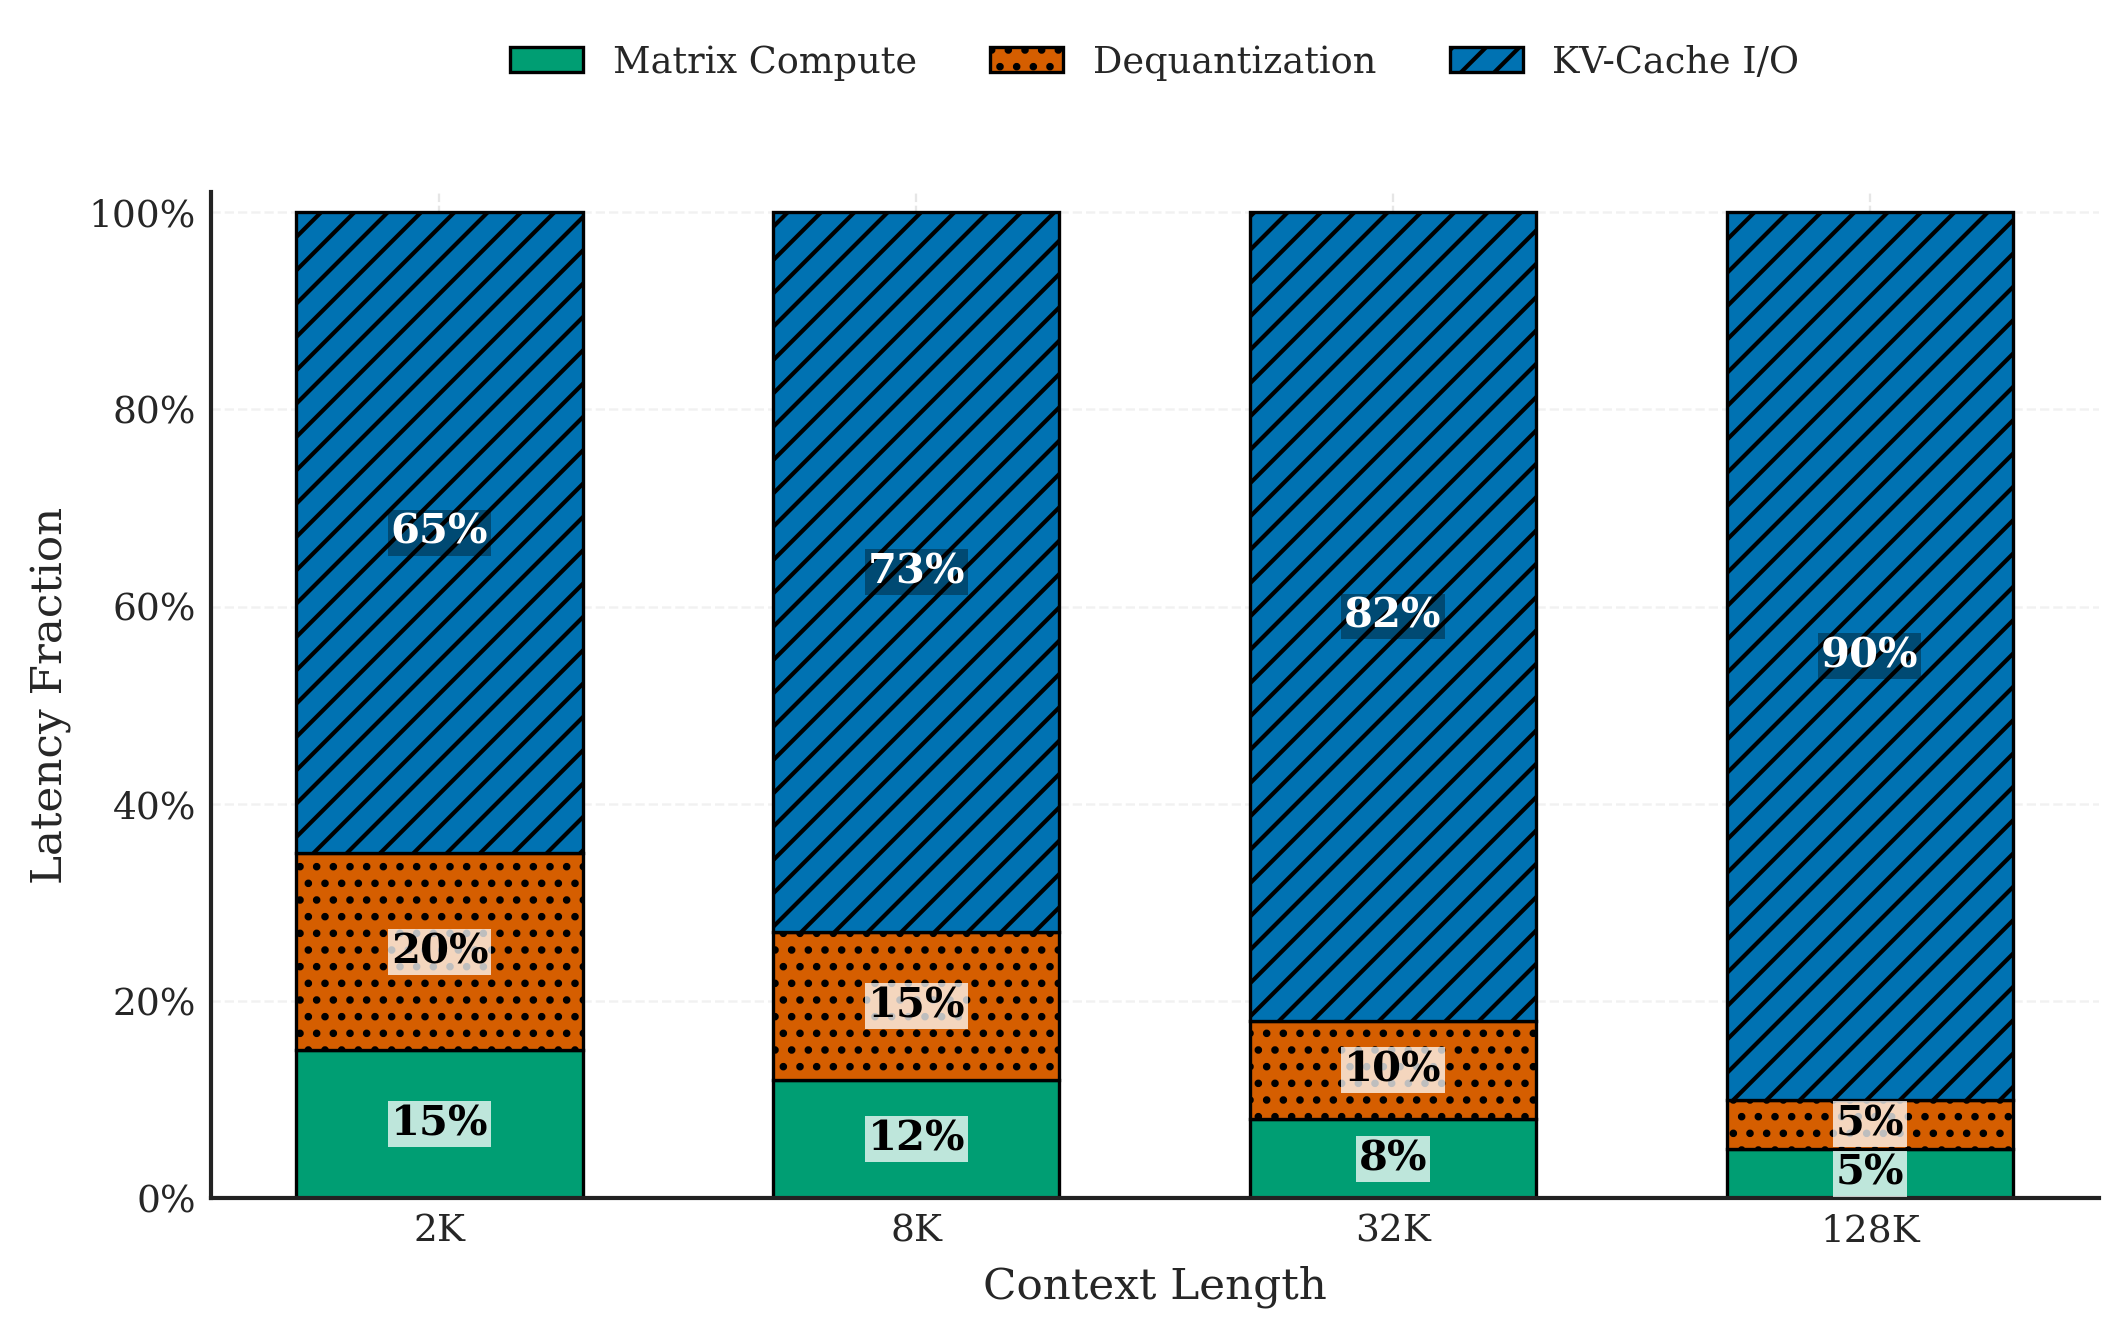
\includegraphics[width=\textwidth]{../paper_assets/figures/fig1_latency_breakdown.png}
\caption[Latency breakdown across context lengths]{Profiler output used to choose design targets, with arithmetic, conversion, and old-token KV service shown separately.}
\label{fig:latency}
\end{figure}

Figure~\ref{fig:latency} shows where the crossover occurs. At 2K and 8K contexts, model arithmetic still occupies a visible part of the total. At 32K and 128K contexts, the bar is mostly historical KV traversal, with format conversion still large enough to matter. I therefore use the profile as a guide for the rest of the design: improving the matrix engine alone would miss the term that grows fastest.

\subsection{The Reality of PIM Format Mismatches}

Moving attention closer to the KV cache addresses only half of the profile. The other half is numeric format. Practical serving stacks often store KV-cache tensors in low precision, for example INT8, to stretch memory capacity~\cite{llm_outliers}. Existing memory-proximate compute engines commonly provide floating-point softmax or other wide nonlinear datapaths~\cite{pim_quant}. If the PIM pipeline has to unpack integer KV data, evaluate the nonlinear stage in floating point, and then repack the result, a significant part of the near-memory advantage is lost to conversion.

\section{Summary}

The evidence in this chapter leaves two design requirements. First, the largest repeated object in the decode loop should not be dragged back to the host whenever a token is generated. Second, the nonlinear portion of attention should not force the cache to leave its compact representation before any useful near-memory work happens. LKC-CXL-PIM addresses these requirements inside one endpoint, and DisaggKV tests the same principles when the cache is spread across a CXL pool.

These requirements become the design checklist used in the next two chapters:
\begin{enumerate}
    \item \textbf{Move work to the cache rather than moving the cache to the host.} The historical KV cache is the repeated state object in long-context decode, so the architecture should minimize host-facing transfers of that state.
    \item \textbf{Keep the common case narrow.} Quantized KV-cache storage is only useful if the memory-side datapath can consume it without expanding ordinary activations into a floating-point pipeline.
    \item \textbf{Synchronize only what must be global.} Distributed attention needs a shared maximum and sum for correct softmax normalization. Those values are scalars, so the multi-node design treats scalar reduction as the natural CXL fabric primitive.
\end{enumerate}

\chapter{LKC-CXL-PIM: Single-Node Architecture}
\label{ch:inlu_architecture}

This chapter describes the single-endpoint artifact, \textbf{LKC-CXL-PIM} (Long KV Cache via CXL Processing-in-Memory). The design is aimed at two costs measured in Chapter~\ref{ch:motivation}: moving historical K/V state back through the host path, and expanding compact KV data only to run a floating-point nonlinear stage.

\section{Request Path at the CXL Endpoint}

In the single-node artifact, the old K/V pages remain in the HBM stack behind the CXL endpoint. A decode step is issued as a descriptor, not as a request to pull the whole historical region back to the host. The descriptor includes the query vector $\mathbf{Q}$, the KV-page range, the head identifier, and the scale metadata used by the integer path. Once the CXL controller forwards it to the logic base die, the endpoint scores keys and accumulates values beside the cache lines that supply the data~\cite{attentionlego}.

For the simulator, I made the endpoint deliberately narrow. It is a memory-side service attached to the KV pages, not a miniature GPU placed behind the CXL port. The reason is mechanical: the object that grows with context length is the HBM-resident KV history. A token step therefore sends in a descriptor and receives back a reduced attention vector. Under that boundary, the logic die needs local integer attention and the small overflow route; it does not need a general tensor core or a floating-point softmax block.

\section{One-Token Walk Through HBM}

The per-token path is short enough to state explicitly. The host schedules the request and runs the non-attention portions of the model. The endpoint handles only the KV range for the token being generated. After the descriptor arrives, local HBM streams key and value cache lines into the logic path. The endpoint computes integer dot products with the query, routes ordinary activations through the INT8 lane, and sends rare high-magnitude values through the overflow path. After the local maximum is found, the iNLU evaluates shifted exponentials and the endpoint updates the exponential sum and weighted-value accumulator.

The live state during the walk is small. The endpoint updates the maximum logit, the exponential sum, and the weighted value accumulator as cache lines arrive. It does not build an attention matrix on the logic die. From the host side, the transaction is intentionally plain: submit the descriptor, let the endpoint traverse its KV pages, and receive the attention result.

\section{Outlier-Aware Routing and Overflow Handling}

The main nuisance in a low-precision attention path is not the average activation; it is the occasional large value. Prior work shows that these outliers are rare but can still dominate quantized Transformer accuracy~\cite{llm_outliers}. That creates a hardware trade-off that shows up directly in this design: a wide datapath sized for the rare value wastes area most of the time, but a narrow datapath that clips those values can change the attention result.

LKC-CXL-PIM handles that case with an \textbf{Outlier-Aware Logic} front-end. The front-end does not try to make every activation expensive; it sorts the common values away from the few high-magnitude values that need more precision.

\begin{figure}[htbp]
\centering
\resizebox{0.9\textwidth}{!}{%
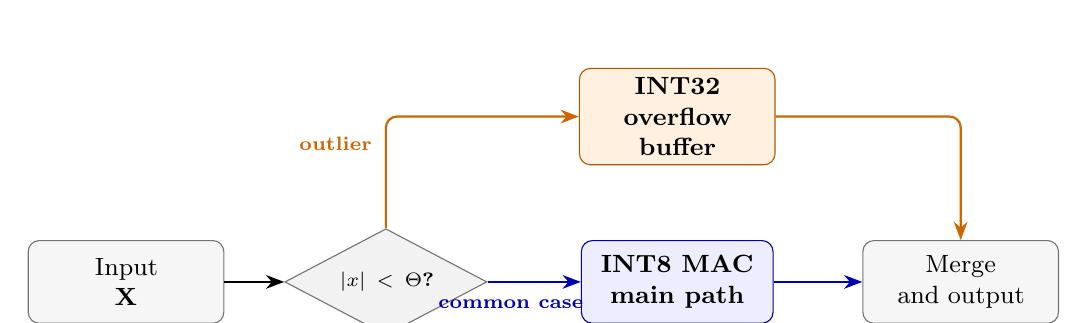
\begin{tikzpicture}[auto, >=Stealth,
    data/.style={rectangle, draw=black!55, fill=gray!7, text width=2.25cm, align=center, rounded corners, minimum height=1.05cm, font=\small},
    branch/.style={diamond, draw=black!55, fill=gray!10, aspect=1.9, text width=2.1cm, align=center, inner sep=0pt, font=\scriptsize\bfseries, minimum height=1.35cm},
    common/.style={rectangle, draw=blue!65!black, fill=blue!7, text width=2.2cm, align=center, rounded corners, minimum height=1.05cm, font=\small\bfseries},
    rare/.style={rectangle, draw=orange!70!black, fill=orange!12, text width=2.25cm, align=center, rounded corners, minimum height=1.05cm, font=\small\bfseries},
    arrow/.style={thick, ->, rounded corners}]

    \node[data] at (0,0) (input) {Input\\$\mathbf{X}$};
    \node[branch] at (3.3,0) (classify) {$|x| < \Theta$?};
    \node[common] at (7.0,0) (int8) {INT8 MAC\\main path};
    \node[rare] at (7.0,2.1) (overflow) {INT32 overflow\\buffer};
    \node[data] at (10.6,0) (merge) {Merge\\and output};

    \draw[arrow] (input) -- (classify);
    \draw[arrow, draw=blue!70!black] (classify) -- node[near start, below=0.1cm, font=\scriptsize\bfseries, text=blue!70!black] {common case} (int8);
    \draw[arrow, draw=orange!80!black] (classify) |- node[pos=0.38, left=0.05cm, font=\scriptsize\bfseries, text=orange!80!black] {outlier} (overflow);
    \draw[arrow, draw=blue!70!black] (int8) -- (merge);
    \draw[arrow, draw=orange!80!black] (overflow) -| (merge);
\end{tikzpicture}
}
\caption[Outlier-aware datapath]{Outlier-aware datapath. Most activations remain on the INT8 path, while rare outliers are redirected to a high-precision overflow buffer.}
\label{fig:outlier}
\end{figure}

Figure~\ref{fig:outlier} illustrates the split. Activations satisfying $|x| < \Theta$ go to the dense INT8 array, while values outside that range are diverted into a small INT32 overflow buffer. The evaluated 16-entry buffer is a compromise: it recovers most of the accuracy lost by a pure INT8 path, but it remains small enough not to dominate the logic-die budget. When the overflow path fills, the local controller stalls, drains the buffered entries, and then resumes. That stall is a correctness backstop rather than the expected steady-state behavior.

\section{Integer Non-Linear Unit (iNLU)}

After the routing decision, the expensive piece is the softmax exponential. A conventional implementation would leave the compact KV path, evaluate the nonlinear operation in floating point, and then return to the narrower representation~\cite{flashattn2, newton_aim}. LKC-CXL-PIM avoids that detour with an \textbf{Integer Non-Linear Unit (iNLU)} that evaluates the approximation in a fixed-point integer domain.

The iNLU begins by rewriting the exponential using a base-2 decomposition:
\begin{equation}
e^x = 2^{x / \ln 2}
\end{equation}
Let
\begin{equation}
n = \left\lfloor \frac{x}{\ln 2} \right\rfloor, \qquad f = x - n \cdot \ln 2
\end{equation}
so that
\begin{equation}
e^x = 2^n \cdot e^f \quad (\text{where } 0 \leq f < \ln 2)
\end{equation}
The constrained interval for $f$ allows the nonlinear term $e^f$ to be approximated with a low-order polynomial rather than a large lookup table:
\begin{equation}
e^f \approx A \cdot {(f + B)}^2 + C
\end{equation}
where $A$, $B$, and $C$ are precomputed constants in the chosen fixed-point format~\cite{llm_int8}.

Table~\ref{tab:synthesis_results} reports the synthesis comparison for the nonlinear unit itself. I keep it separate from the full-system evaluation because the iNLU is only one block in the endpoint. The table answers a more local question: whether the softmax logic can stay small enough that the benefit of moving computation near memory is not lost to a newly introduced floating-point unit.

\begin{table}[htbp]
\centering
\caption[Softmax-unit synthesis comparison]{Hardware synthesis comparison of the nonlinear unit only: iNLU versus a conventional FP16 softmax unit (TSMC 7\,nm, 1\,GHz target).}
\label{tab:synthesis_results}
\begin{tabular}{lccc}
\toprule
\textbf{Metric} & \textbf{FP16 Softmax (Baseline)} & \textbf{iNLU (Ours)} & \textbf{Savings} \\
\midrule
Gate Count (K)          & 118.4  & 24.2   & 79.5\% \\
Die Area (mm$^2$)       & 0.0461 & 0.0094 & 79.6\% \\
Dynamic Power (mW)      & 17.8   & 3.6    & 79.8\% \\
Max Frequency (GHz)     & 0.95   & 1.32   & 38.9\% \\
\bottomrule
\end{tabular}
\end{table}

\begin{figure}[htbp]
\centering
\resizebox{0.9\textwidth}{!}{%
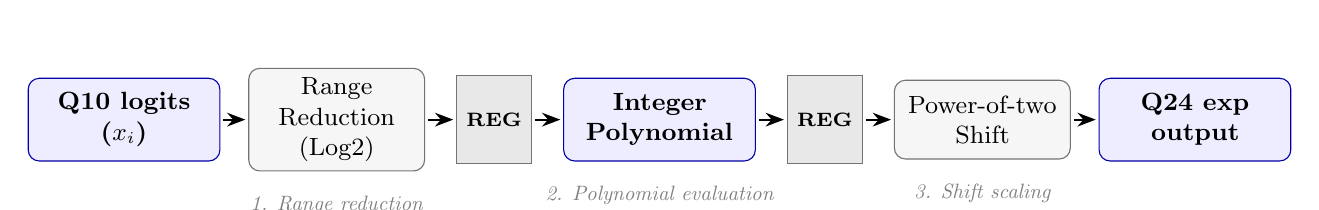
\begin{tikzpicture}[auto, >=Stealth,
    block/.style={rectangle, draw=blue!65!black, fill=blue!7, text width=2.2cm, align=center, rounded corners, minimum height=1.05cm, font=\small\bfseries},
    logic/.style={rectangle, draw=black!55, fill=gray!7, text width=2.0cm, align=center, rounded corners, minimum height=1.0cm, font=\small},
    reg/.style={rectangle, draw=black!55, fill=gray!18, text width=0.72cm, align=center, minimum height=1.12cm, font=\scriptsize\bfseries},
    arrow/.style={->, thick, shorten >=1pt, shorten <=1pt}]

    \node [block] at (0,0) (input) {Q10 logits\\($x_i$)};
    \node [logic] at (2.7,0) (log2) {Range \\ Reduction \\ (Log2)};
    \node [reg]   at (4.7,0) (r1) {REG};
    \node [block] at (6.8,0) (poly) {Integer \\ Polynomial};
    \node [reg]   at (8.9,0) (r2) {REG};
    \node [logic] at (10.9,0) (denorm) {Power-of-two \\ Shift};
    \node [block] at (13.6,0) (output) {Q24 exp \\ output};

    \draw [arrow] (input) -- (log2);
    \draw [arrow] (log2) -- (r1);
    \draw [arrow] (r1) -- (poly);
    \draw [arrow] (poly) -- (r2);
    \draw [arrow] (r2) -- (denorm);
    \draw [arrow] (denorm) -- (output);

    \node[below=0.22cm of log2.south, font=\itshape\color{gray}, scale=0.75] {1. Range reduction};
    \node[below=0.22cm of poly.south, font=\itshape\color{gray}, scale=0.75] {2. Polynomial evaluation};
    \node[below=0.22cm of denorm.south, font=\itshape\color{gray}, scale=0.75] {3. Shift scaling};
\end{tikzpicture}%
}
\caption[iNLU pipeline architecture]{Pipeline organization of the Integer Non-Linear Unit (iNLU).}
\label{fig:inlu}
\end{figure}

Figure~\ref{fig:inlu} shows the resulting datapath. In the checked model, the iNLU is split into four fixed-point stages: range reduction for the quotient and residual of $x / \ln 2$, construction of the shifted residual term, quadratic polynomial evaluation, and final power-of-two scaling. The last operation is deliberately implemented as a shift, so the endpoint does not reintroduce the floating-point multiply that the design is trying to avoid.

\section{Fixed-Point Error Checks}

The fixed-point check starts at the same point as the software reference: after maximum subtraction. In this artifact the iNLU receives Q10 logits and returns Q24 normalized outputs. That split came from the reduction path rather than from a preference for round numbers. The accumulator needs extra fractional detail once exponentials are summed, but the endpoint should still remain an integer datapath. The constants are therefore tied to the Qwen2.5-7B-Instruct trace setup used here, not proposed as a universal format.

I check the error budget in two places. Inside the iNLU, range reduction clamps values outside the calibrated interval before polynomial evaluation; the golden model stores $\ln 2$ as 710 in Q10 and uses the quadratic triplet $(367, 1385, 352)$. Before the iNLU, the classifier catches high-magnitude activations that could change either the local maximum or the weighted value sum.

Most activations still take the dense INT8 lane. I reserve the overflow buffer for samples that can actually move the attention output, which is why the evaluation looks at the final weighted vector instead of treating the exponential approximation as an isolated microbenchmark.

The accuracy comparison is made at the attention output, not by demanding bitwise equality against FP32 softmax. A smaller nonlinear unit is useful only when the final weighted vector remains close to the reference. Chapter~\ref{ch:evaluation} therefore reports both softmax-level mean-squared error and vector-level cosine similarity. A scalar exponential test would be too narrow, because a small local approximation error can still perturb the weighted value vector.

The classifier and the iNLU are paired for this reason. The classifier keeps the common datapath compact without discarding rare large values, and the iNLU keeps the nonlinear stage in the integer path. The evaluation later measures what changes when that work remains inside the CXL-attached memory stack instead of returning to the host-facing side.

\chapter{DisaggKV: Multi-Node Serving System}
\label{ch:disaggkv_system}

LKC-CXL-PIM covers the one-host, one-endpoint case. A serving cluster adds two complications that the single-endpoint design does not see. First, many requests can share a prompt prefix before their decode histories diverge. Second, the total KV footprint can exceed one endpoint, so a token may need state stored on several CXL-attached memory devices. \textbf{DisaggKV} is the distributed design I use for that setting: it places KV pages according to reuse and performs the softmax reduction inside the endpoint group.

\section{Overview of Multi-Tenant Disaggregation}

\begin{figure}[htbp]
\centering
\resizebox{0.82\textwidth}{!}{%
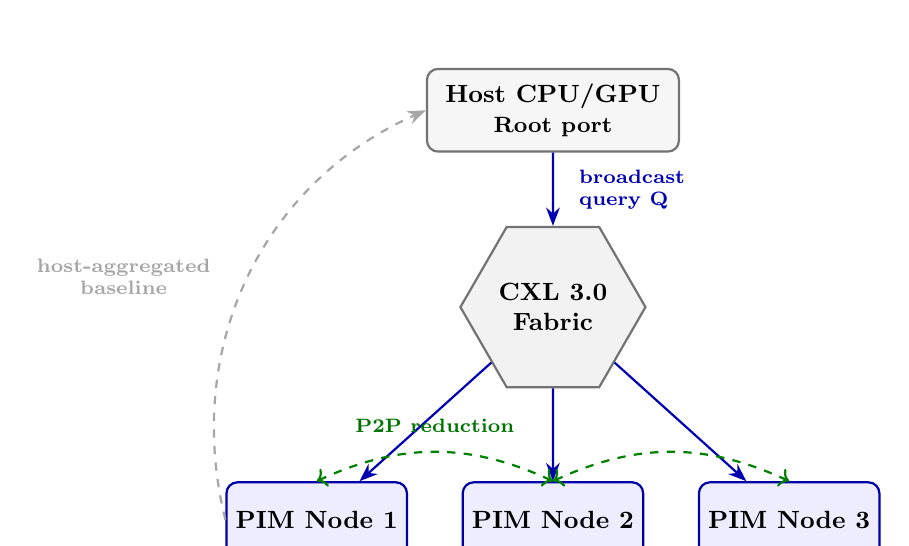
\begin{tikzpicture}[
    host/.style={rectangle, draw=black!55, fill=gray!7, thick, minimum width=3.2cm, minimum height=1.05cm, align=center, rounded corners, font=\small\bfseries},
    switch/.style={regular polygon, regular polygon sides=6, draw=black!55, fill=gray!10, thick, minimum size=2.35cm, inner sep=0pt, align=center, font=\small\bfseries},
    pim/.style={rectangle, draw=blue!65!black, fill=blue!7, thick, minimum width=2.1cm, minimum height=0.95cm, align=center, rounded corners, font=\small\bfseries},
    arrow/.style={thick, -Stealth}
]
    \node[host] (host) at (0,0) {Host CPU/GPU\\{\footnotesize Root port}};
    \node[switch] (switch) at (0,-2.5) {CXL 3.0\\Fabric};

    \node[pim] (n1) at (-3.0,-5.2) {PIM Node 1};
    \node[pim] (n2) at (0,-5.2) {PIM Node 2};
    \node[pim] (n3) at (3.0,-5.2) {PIM Node 3};

    \draw[arrow, draw=blue!70!black] (host) -- node[right=0.2cm, font=\scriptsize\bfseries, text=blue!70!black, align=left] {broadcast\\query $\mathbf{Q}$} (switch);
    \draw[arrow, draw=blue!70!black] (switch) -- (n1);
    \draw[arrow, draw=blue!70!black] (switch) -- (n2);
    \draw[arrow, draw=blue!70!black] (switch) -- (n3);

    \draw[arrow, dashed, draw=gray!70, bend left=40] (n1.west) to node[midway, left=0.35cm, font=\scriptsize\bfseries, text=gray!70, align=center] {host-aggregated\\baseline} (host.west);
    \draw[<->, thick, dashed, draw=green!50!black] (n1.north) to[bend left=25] node[midway, above=0.12cm, font=\scriptsize\bfseries, text=green!45!black] {P2P reduction} (n2.north);
    \draw[<->, thick, dashed, draw=green!50!black] (n2.north) to[bend left=25] (n3.north);
\end{tikzpicture}
}
\caption[DisaggKV system overview]{Architectural overview of DisaggKV\@. Query vectors are broadcast from the host, while distributed softmax barriers are exchanged directly among CXL-attached PIM nodes.}
\label{fig:disaggkv_overview}
\end{figure}

Figure~\ref{fig:disaggkv_overview} marks the main difference from the baseline. In the host-aggregated path, partial attention state returns through the Root Complex before consolidation. Long-context decode then stresses the same host-facing links and switch ports that already limit CXL memory pooling~\cite{cxl_pond}. DisaggKV keeps the host as the scheduler and final consumer, but the maximum and sum needed by softmax are exchanged directly among endpoints.

\section{Hypervisor Locality-Aware Paging}

The generated serving trace gives each page a reuse label. Prefix pages can be read by many sessions, while continuation pages usually become private once generation starts. I feed that label into the placement policy because the two page types have different failure modes: copying a prefix page duplicates shared state, while chasing a private page around the pool creates traffic that rarely pays back later~\cite{splitwise}.

The allocator uses the label directly. Reused prefix pages go to shared nodes so later sessions can attach to the same copy. Continuation pages are spread across the remaining endpoints, mostly to avoid one endpoint becoming the private-history sink. The migration daemon waits until imbalance is persistent before moving private pages, which keeps short-lived rebalancing traffic out of the common path.

Algorithm~\ref{alg:placement} gives the placement rule used by the simulator. The policy is intentionally simple because the report is not trying to invent a full cloud scheduler. Its purpose is to expose the architectural effect of keeping reusable prefix state stable while distributing private continuation state enough to prevent one endpoint from becoming the capacity or service bottleneck.

\begin{algorithm}[htbp]
\caption{Locality-aware KV-page placement}
\label{alg:placement}
\begin{algorithmic}[1]
\FOR{each newly allocated KV page}
    \IF{the page belongs to a shared prompt prefix}
        \STATE Place it on the least-loaded node in the shared-prefix group.
        \STATE Record the prefix identifier so later requests can reuse the same page.
    \ELSE
        \STATE Place it on the least-loaded private node for the owning request.
        \STATE Bind future continuation pages from the same request to nearby nodes.
    \ENDIF
\ENDFOR
\STATE Periodically rebalance only when private-node load exceeds the migration threshold.
\end{algorithmic}
\end{algorithm}

The same rule also keeps metadata movement modest. Prefix pages stay stable because many sessions may reference them, while private pages are allowed to spread because they mostly serve one request. In the modeled workload, this distinction keeps page movement small enough that migration traffic does not drown out the peer-to-peer reduction traffic.

\section{Peer-to-Peer Fabric Synchronization}

Capacity pooling alone does not make sharded attention correct. If each endpoint normalizes only its own logits, the probability mass is split across incompatible local views. Every shard needs the same maximum logit and the same exponential sum before it can produce a normalized contribution~\cite{ring_attention}.

DisaggKV obtains those two values with an endpoint-side two-step reduction. The exchange is deliberately narrow: it does not ship partial tensors when two scalars are enough for stable softmax. In the first phase, each node reports its largest local logit $L_{\max}$, and the endpoint group agrees on \texttt{Global\_Max}. In the second phase, each node evaluates exponentials relative to that shared maximum, contributes its local sum, and receives the final \texttt{Global\_Sum}.

\begin{figure}[htbp]
\centering
\resizebox{0.86\textwidth}{!}{%
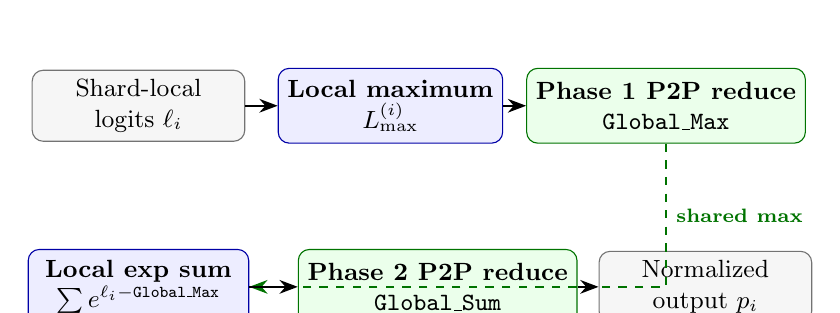
\begin{tikzpicture}[
    node distance=1.0cm and 1.0cm,
    data/.style={rectangle, draw=black!55, fill=gray!7, rounded corners, minimum width=2.7cm, minimum height=0.9cm, align=center, font=\small},
    stage/.style={rectangle, draw=blue!65!black, fill=blue!7, rounded corners, minimum width=2.8cm, minimum height=0.95cm, align=center, font=\small\bfseries},
    sync/.style={rectangle, draw=green!45!black, fill=green!8, rounded corners, minimum width=3.1cm, minimum height=0.95cm, align=center, font=\small\bfseries},
    arrow/.style={-Stealth, thick},
    soft/.style={-Stealth, thick, dashed, draw=green!45!black}
]
    \node[data] (logits) at (0,1.2) {Shard-local\\logits $\ell_i$};
    \node[stage] (localmax) at (3.2,1.2) {Local maximum\\$L_{\max}^{(i)}$};
    \node[sync] (gmax) at (6.7,1.2) {Phase 1 P2P reduce\\\texttt{Global\_Max}};

    \node[stage] (localsum) at (0,-1.1) {Local exp sum\\$\sum e^{\ell_i-\texttt{Global\_Max}}$};
    \node[sync] (gsum) at (3.8,-1.1) {Phase 2 P2P reduce\\\texttt{Global\_Sum}};
    \node[data] (output) at (7.2,-1.1) {Normalized\\output $p_i$};

    \draw[arrow] (logits) -- (localmax);
    \draw[arrow] (localmax) -- (gmax);
    \draw[soft] (gmax.south) |- node[pos=0.25, right, font=\scriptsize\bfseries, text=green!45!black] {shared max} (localsum.east);
    \draw[arrow] (localsum) -- (gsum);
    \draw[arrow] (gsum) -- (output);
\end{tikzpicture}%
}
\caption[Two-phase peer-to-peer reduction]{Two-phase peer-to-peer reduction in DisaggKV\@. Nodes first exchange the global maximum for numerically stable exponentiation, then exchange the global exponential sum before final normalization.}
\label{fig:reduction_protocol}
\end{figure}

Figure~\ref{fig:reduction_protocol} summarizes the exchange. During the two barriers, only scalar state crosses the fabric, so the evaluated synchronization traffic is measured in kilobytes per decode step. This does not make synchronization free; the endpoints still wait at barriers. It does, however, change the synchronized object from dense KV-derived tensors to the minimum state needed for numerically correct normalization.

\section{Epoch Rules for Missing Shards}

The endpoint group treats each decode step as a short synchronization epoch. During that epoch, every participating node reads a fixed KV-page snapshot and contributes to the same \texttt{Global\_Max} and \texttt{Global\_Sum}. New page allocations are installed only at epoch boundaries, so the reduction protocol does not have to handle a page moving while a token is being normalized.

The epoch tag is not just bookkeeping. It is the rule that prevents a late shard from being counted in the wrong token. If one endpoint reaches the barrier after the others, the group waits for that epoch instead of folding the payload into the next normalization window. In the injected-fault runs, a degraded node loses the reduction payload for that same tag, and the parity-assisted path rebuilds it before the group advances. I keep the fault model narrow: transient sub-flit loss and short endpoint stalls are included, but permanent loss of a memory-pool device is left to a runtime recovery layer outside this artifact.

\section{Clock-Crossing Buffer at the Endpoint}

The CXL-fabric model does not deliver all shard messages in lockstep. Queueing delay and packet-time variation mean that two endpoints can reach the same barrier at slightly different simulated times. Without a boundary buffer, packet jitter, transient congestion, or clock-domain mismatch would show up directly as disruption in the reduction pipeline~\cite{hpc_network}. DisaggKV places asynchronous FIFOs at the endpoint boundary so short timing skew is absorbed before it becomes PIM-side back-pressure.

The FIFO is sized as a boundary buffer, not as a congestion reservoir. It separates fabric timing from endpoint timing and lets the local pipeline absorb short bursts through a Gray-coded clock-domain crossing. If the barrier is still late after that buffering, the endpoint stalls its own reduction state rather than immediately escalating to the host. The parity repair path uses the same boundary: missing sub-flits can be repaired locally, while coarse restart is reserved for failures beyond the modeled scope~\cite{cxl_memory_failure}.

\chapter{Experimental Methodology}
\label{ch:methodology}

The evaluation uses several models because the artifact spans different time scales. HBM row timing needs a cycle-level memory simulator. Multi-endpoint CXL behavior needs an event model with queues and switch-port service limits. The nonlinear datapath is better represented by synthesis-derived proxy numbers than by a memory simulator. This chapter records how those pieces meet, since the reported curves mix direct counters with calibrated estimates only where the connection is explicit.

\section{Simulation Infrastructure}

I use the simulators for different jobs. The customized \textbf{Ramulator 2.0} setup is responsible for single-node timing, including bank timing, row-buffer behavior, and the added PIM commands~\cite{ramulator2}. The Python event model is responsible for multi-node CXL behavior: packet routing, endpoint synchronization, and shared-link queues. The two parts meet through the measured endpoint service cost from the single-node run, so the cluster model does not rely on a manually selected speedup constant.

\subsection{Memory and PIM Modeling}

The single-node substrate is HBM3 at a 2\,GHz memory clock. The Ramulator command set is extended with PIM operations for the integer compute path and the overflow path. For arithmetic validation, the iNLU is compared against a fixed-point golden model with Q10 logits, integer polynomial exponentiation, and Q24 normalization. The outlier-routing block is checked against the SystemVerilog implementation. Area and power are used as synthesis-derived proxy inputs; I do not present them as a completed place-and-route result.

\subsection{CXL Fabric Topology Emulator}

Distributed execution across multiple PIM nodes is evaluated using an event-driven CXL-fabric simulator wrapped around the single-node timing model. Table~\ref{tab:sim_params} summarizes the principal system parameters used in the thesis.

\begin{table}[htbp]
\centering
\caption[Simulation parameters]{System simulation parameters used for the memory and CXL-fabric models.}
\label{tab:sim_params}
\begin{tabular}{llc}
\toprule
\textbf{Category} & \textbf{Parameter} & \textbf{Value} \\
\midrule
\multirow{3}{*}{Memory (HBM3)} & Base Clock / Data Rate & 2.0 GHz / 4.0 Gbps \\
                              & Channel Bandwidth      & 819 GB/s \\
                              & tCAS / tRP / tRCD     & 14.5 / 14.5 / 14.5 ns \\
\midrule
\multirow{3}{*}{CXL 3.0 Fabric} & Link Width / Latency  & x16 (Gen6) / 150 ns \\
                              & Switch Port BW        & 64 GB/s (Bi-dir) \\
                              & Topology              & Star \\
\bottomrule
\end{tabular}
\end{table}

The distributed simulator supports star and fat-tree topologies, explicit switch-port service limits, and queueing delay at shared links. The reported artifact uses the star topology from the checked-in CXL configuration. I chose the plainer topology because the comparison should be about the data path: host aggregation and peer-to-peer DisaggKV see the same bandwidth and base-latency assumptions.

The curves in Chapter~\ref{ch:evaluation} are not taken from a single opaque simulator output. For each topology, the event model first records bytes moved, service events, and switch-port occupancy. A later queueing pass folds in three calibration inputs: the 128K-token Ramulator read-latency delta, the average switch delay used by the fabric model, and the KV-cache I/O share measured in the 128K latency breakdown. I keep those intermediate values next to the plotted numbers so that a changed curve can be traced to traffic, service time, or one of the calibration constants.

\section{Baseline Rows in the Data Files}

In \path{simulation_results.csv}, the baseline label means that the memory tier is larger, but attention still finishes outside the memory device. The baseline and LKC-CXL-PIM rows use the same 2K--128K decode traces and the same cache-footprint estimates. The controlled difference is the reduction point. The baseline brings K/V traffic back through the host-facing path before the attention result exists; LKC-CXL-PIM performs the local cache walk and reduction at the endpoint, then returns the compact response over CXL.

The cluster-level comparison follows the same rule. Fabric knobs, request arrivals, and endpoint timing are held fixed. The baseline sends partial attention state through the host-facing path; DisaggKV keeps the scalar reductions inside the endpoint group. I do not claim this covers every production optimization. It isolates one data-path decision under the same workload and fabric assumptions.

\section{Workloads and Analytical Traces}

The workload model is derived from a \textbf{Qwen2.5-7B-Instruct} configuration. I use two trace families because one trace shape is not enough to exercise both artifacts:
\begin{itemize}
    \item \textbf{Single-Node Traces:} Decode traces are evaluated at 2K, 8K, 32K, 64K, and 128K context lengths. These traces drive the cycle-accurate comparison between the host-aggregated baseline and LKC-CXL-PIM.
    \item \textbf{Multi-Tenant Traces:} The distributed experiments use Poisson arrival rates from 10 to 50 requests/s with 50 concurrent virtual users. Requests include shared prefixes up to 8K tokens long and user-private dialogue history, allowing the placement policy to see both shared and private access patterns.
\end{itemize}

\section{Recovery Timing under Injected Faults}

Fault timing is measured from injector event to the next point where the endpoint group can continue the modeled reduction. The injector assumes a 3600\,s mean time between failures and includes transient link disruption plus degraded-node behavior. Host-level RDMA backup and checkpoint-restart are included as heavier reference paths; they are intentionally not tuned to look competitive with local parity repair.

\section{Where the Numbers Come From}

Most plotted numbers are regenerated from files committed with the artifact. The file \path{simulation_results.csv} supplies the single-node tables. The file \path{paper_assets/data/paper_metrics.json} stores distributed simulator counters together with the queueing assumptions. Fixed-point softmax and attention-quality figures come from validation outputs under \path{paper_assets/data/}. I keep these sources separate so the report does not blur direct simulator counters with calibrated estimates.

The figures are regenerated by project scripts before they are included in the report. If a future run changes the raw counters, the thesis text should change together with the data summaries. I kept that rule during editing because it prevents the document from drifting away from the artifact and leaves an auditable path from trace generation to plotted result.

\section{Limits of the Evidence}

This section is where I draw the line around the evidence. The area and power tables describe the nonlinear datapath and logic-die budget at the level of synthesis-derived estimates; they are not signoff numbers from placement and routing. The distributed simulator includes the CXL service limits, switch queues, reduction traffic, 50 virtual users, and the star topology used in the checked configuration. It leaves out vendor controller details, firmware scheduling policy, NUMA placement, and operating-system interrupt behavior. The model-quality evidence is also deliberately small: it checks softmax fidelity and a lightweight attention-output comparison, but it is not a substitute for full perplexity or downstream-task evaluation on a production LLM.

Inside that envelope, the runs point in one direction. Less KV-derived data returns through the host-facing path, and the tail-latency knee moves to a higher request rate. I stop the claim there. A prototype would be needed before making stronger statements about operating-system overheads, controller firmware behavior, thermal limits, or model-quality impact.

Taken together, the methodology is hybrid but traceable: cycle-level memory timing for the single-node path, event-driven queueing and synchronization for the distributed path, and synthesis-derived proxy estimates for logic-level efficiency trends.

\chapter{System Evaluation}
\label{ch:evaluation}

This chapter reports the quantitative results for the two artifacts. I separate the single-node and distributed results because they answer different questions. LKC-CXL-PIM asks how much decode work can be moved into one CXL-attached HBM endpoint. DisaggKV asks whether the same traffic reduction remains useful when the KV cache is distributed across endpoints. Table~\ref{tab:results_summary} gives the single-node counters that are used repeatedly in the discussion.

\begin{table}[htbp]
\centering
\caption[Summary of single-node results]{Summary of quantitative single-node results for the baseline and LKC-CXL-PIM.}
\label{tab:results_summary}
\begin{tabular}{lcccc}
\toprule
\textbf{Context Length} & \textbf{Metric} & \textbf{Baseline} & \textbf{LKC-CXL-PIM} & \textbf{Improvement} \\
\midrule
\multirow{2}{*}{8K}   & Read Latency (M Cycles) & 10.77 & 0.12 & 91.5$\times$ \\
                      & Row Misses              & 80,483 & 1,195 & 67.3$\times$ \\
\midrule
\multirow{2}{*}{128K} & Read Latency (M Cycles) & 77.90 & 0.80 & 98.0$\times$ \\
                      & Row Misses              & 288,535 & 3,700 & 78.0$\times$ \\
\midrule
\textbf{Overall}      & Logic Area (Relative)   & 1.00 & 0.83 & 17\% Savings \\
\bottomrule
\end{tabular}
\end{table}

\section{Single-Node Performance Speedup}

\begin{figure}[htbp]
\centering
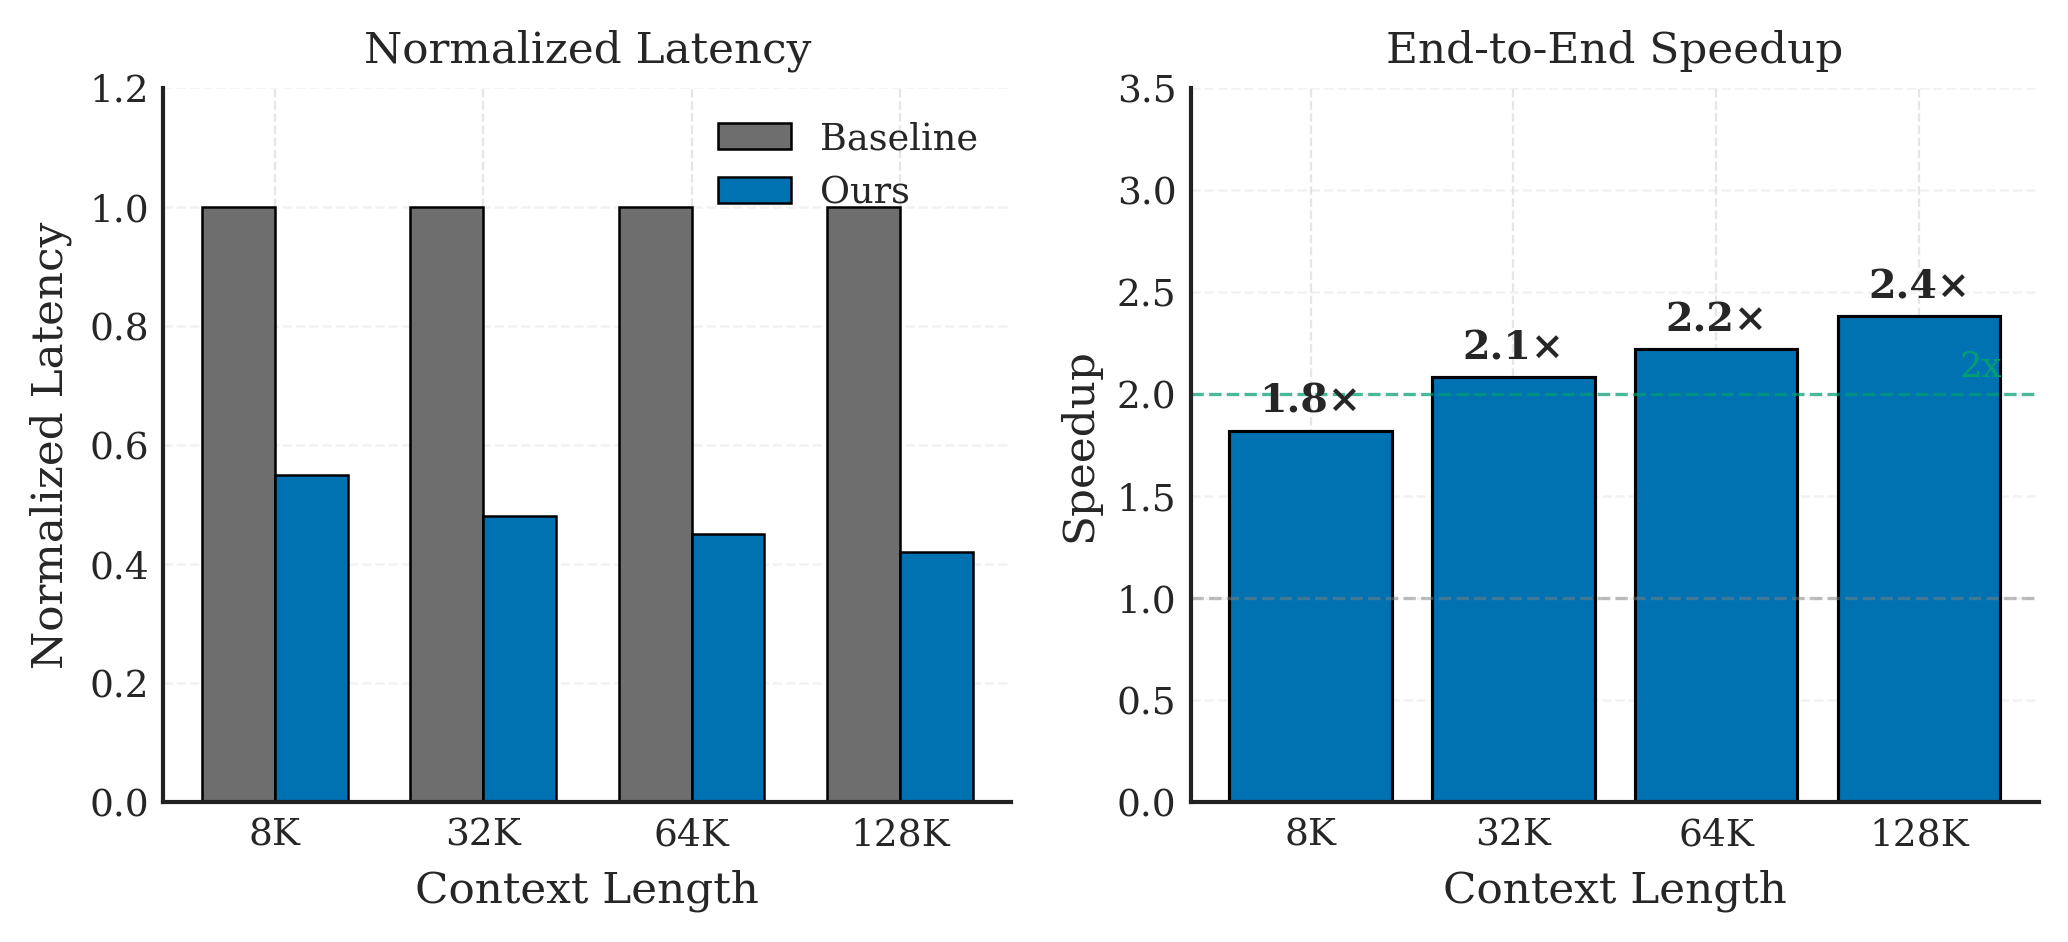
\includegraphics[width=\textwidth]{../paper_assets/figures/fig5_performance_speedup.png}
\caption[Single-node decode speedup]{End-to-end decode speedup of LKC-CXL-PIM relative to the host-aggregated baseline across context lengths.}
\label{fig:performance_speedup}
\end{figure}

Figure~\ref{fig:performance_speedup} reports end-to-end decode speedup. The trend is more important than the absolute value: as context length grows, a larger fraction of the baseline runtime is spent moving KV-cache data rather than computing on it. The measured speedup rises from $1.8\times$ at 8K to $2.4\times$ at 128K, which matches the expectation from the trace profile in Chapter~\ref{ch:motivation}.

\begin{figure}[htbp]
\centering
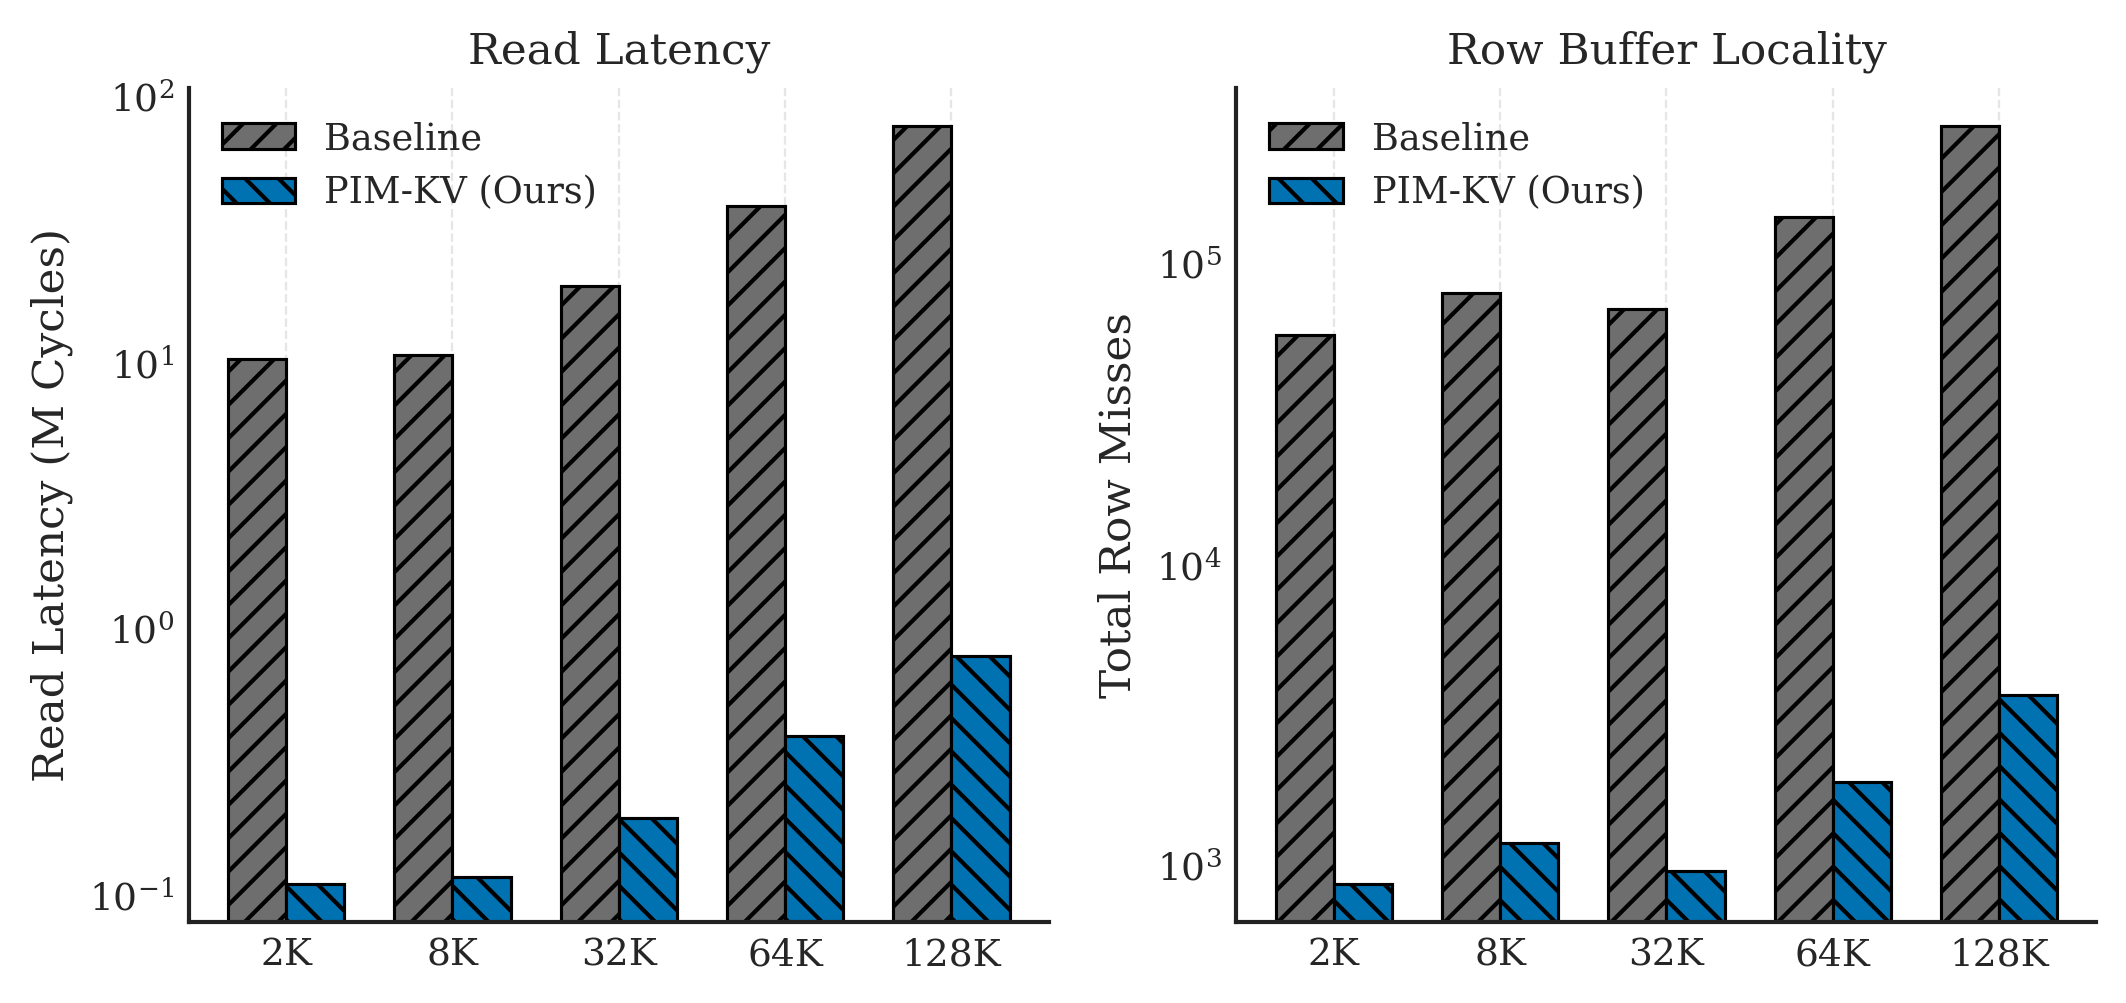
\includegraphics[width=0.9\textwidth]{../paper_assets/figures/fig7_ramulator_comparison.png}
\caption[Cycle-accurate latency comparison]{Cycle-accurate comparison of latency components and row-buffer locality for the baseline and LKC-CXL-PIM.}
\label{fig:ramulator}
\end{figure}

Figure~\ref{fig:ramulator} shows the source of that speedup. At 8K context length, read latency drops from 10.77\,M cycles to 0.12\,M cycles. At 128K, it drops from 77.90\,M cycles to 0.80\,M cycles. The same reorganization also improves row-buffer locality: row misses fall from 80,483 to 1,195 at 8K and from 288,535 to 3,700 at 128K. These reductions are consistent with the intended design goal of keeping KV-cache accesses local to the memory device. They also explain why the result improves with context length: the baseline repeats a larger remote traversal, while LKC-CXL-PIM keeps most of that traversal inside the endpoint.

The difference between the nearly two-order-of-magnitude memory-counter reduction and the more modest end-to-end speedup is expected. Decode still contains non-KV work, host scheduling overhead, and residual synchronization cost. LKC-CXL-PIM therefore does not make generation free; it removes the term that grows most aggressively with context length. This distinction is important because it prevents the memory results from being mistaken for a full application-level speedup.

\section{Area and Energy Efficiency}

\begin{figure}[htbp]
    \centering
    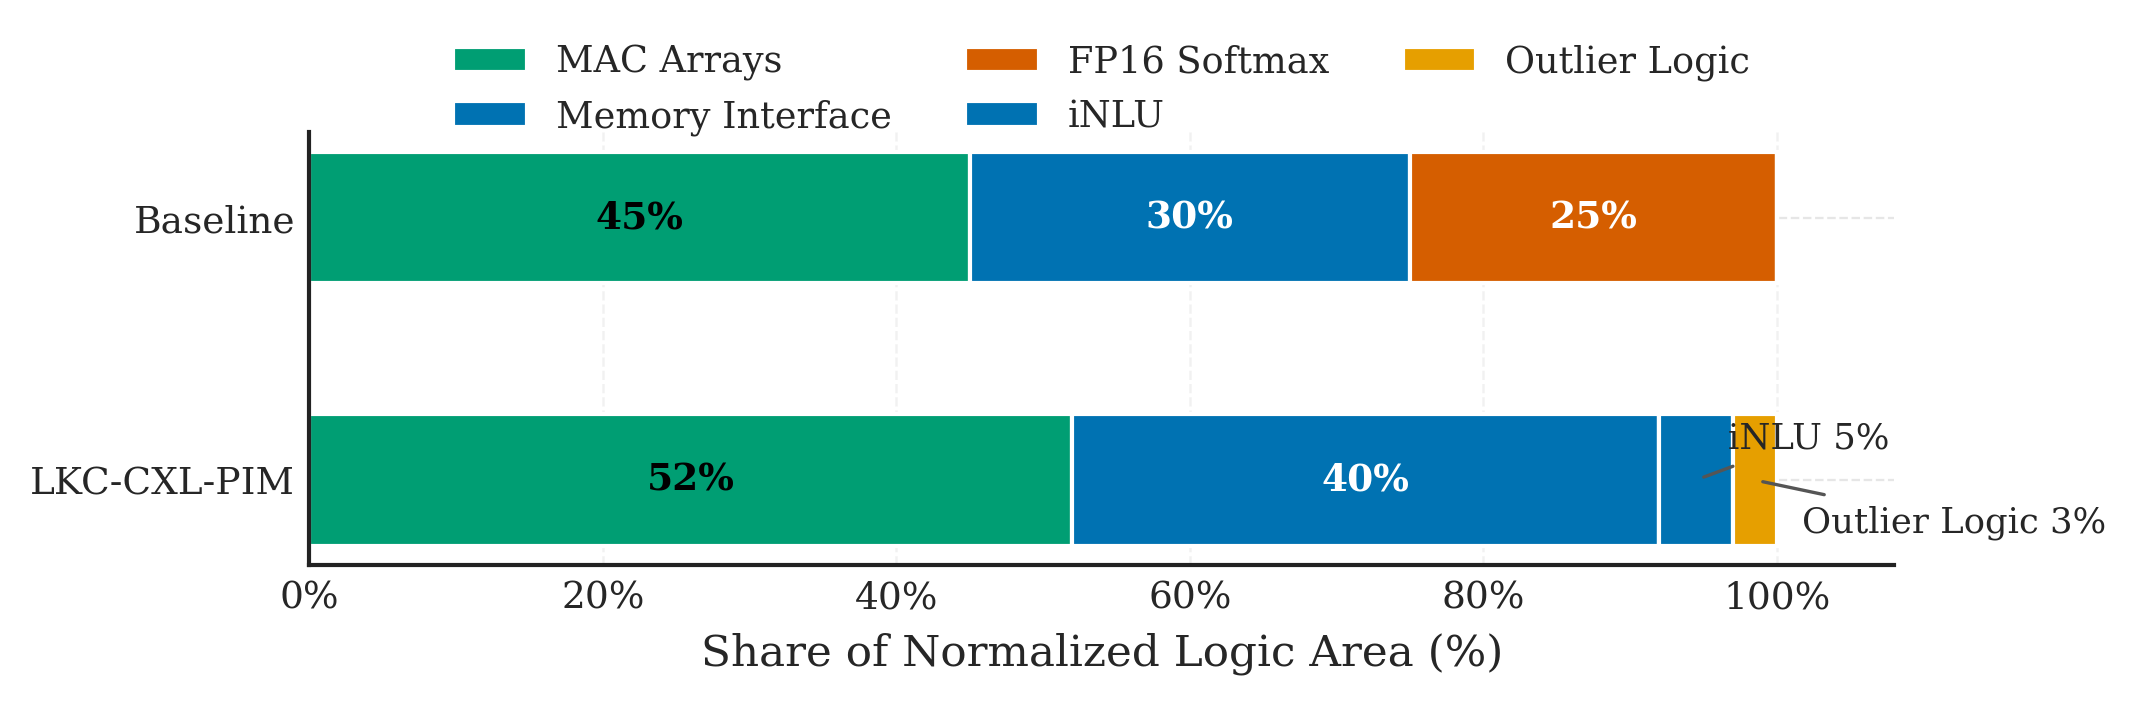
\includegraphics[width=0.92\textwidth]{../paper_assets/figures/fig6_area_breakdown.png}
    \caption[Overall area breakdown]{Overall logic-area breakdown for the baseline softmax path and the LKC-CXL-PIM datapath.}
    \label{fig:area}
\end{figure}

Figure~\ref{fig:area} reports the area breakdown at the logic-die level. In the baseline organization, the FP16 softmax block occupies approximately 25\% of the logic budget. In LKC-CXL-PIM, that block is replaced by the iNLU and outlier-handling path, whose combined footprint is approximately 8\%. The net result is a 17\% overall logic-area reduction even after adding the overflow path.

\begin{figure}[htbp]
    \centering
    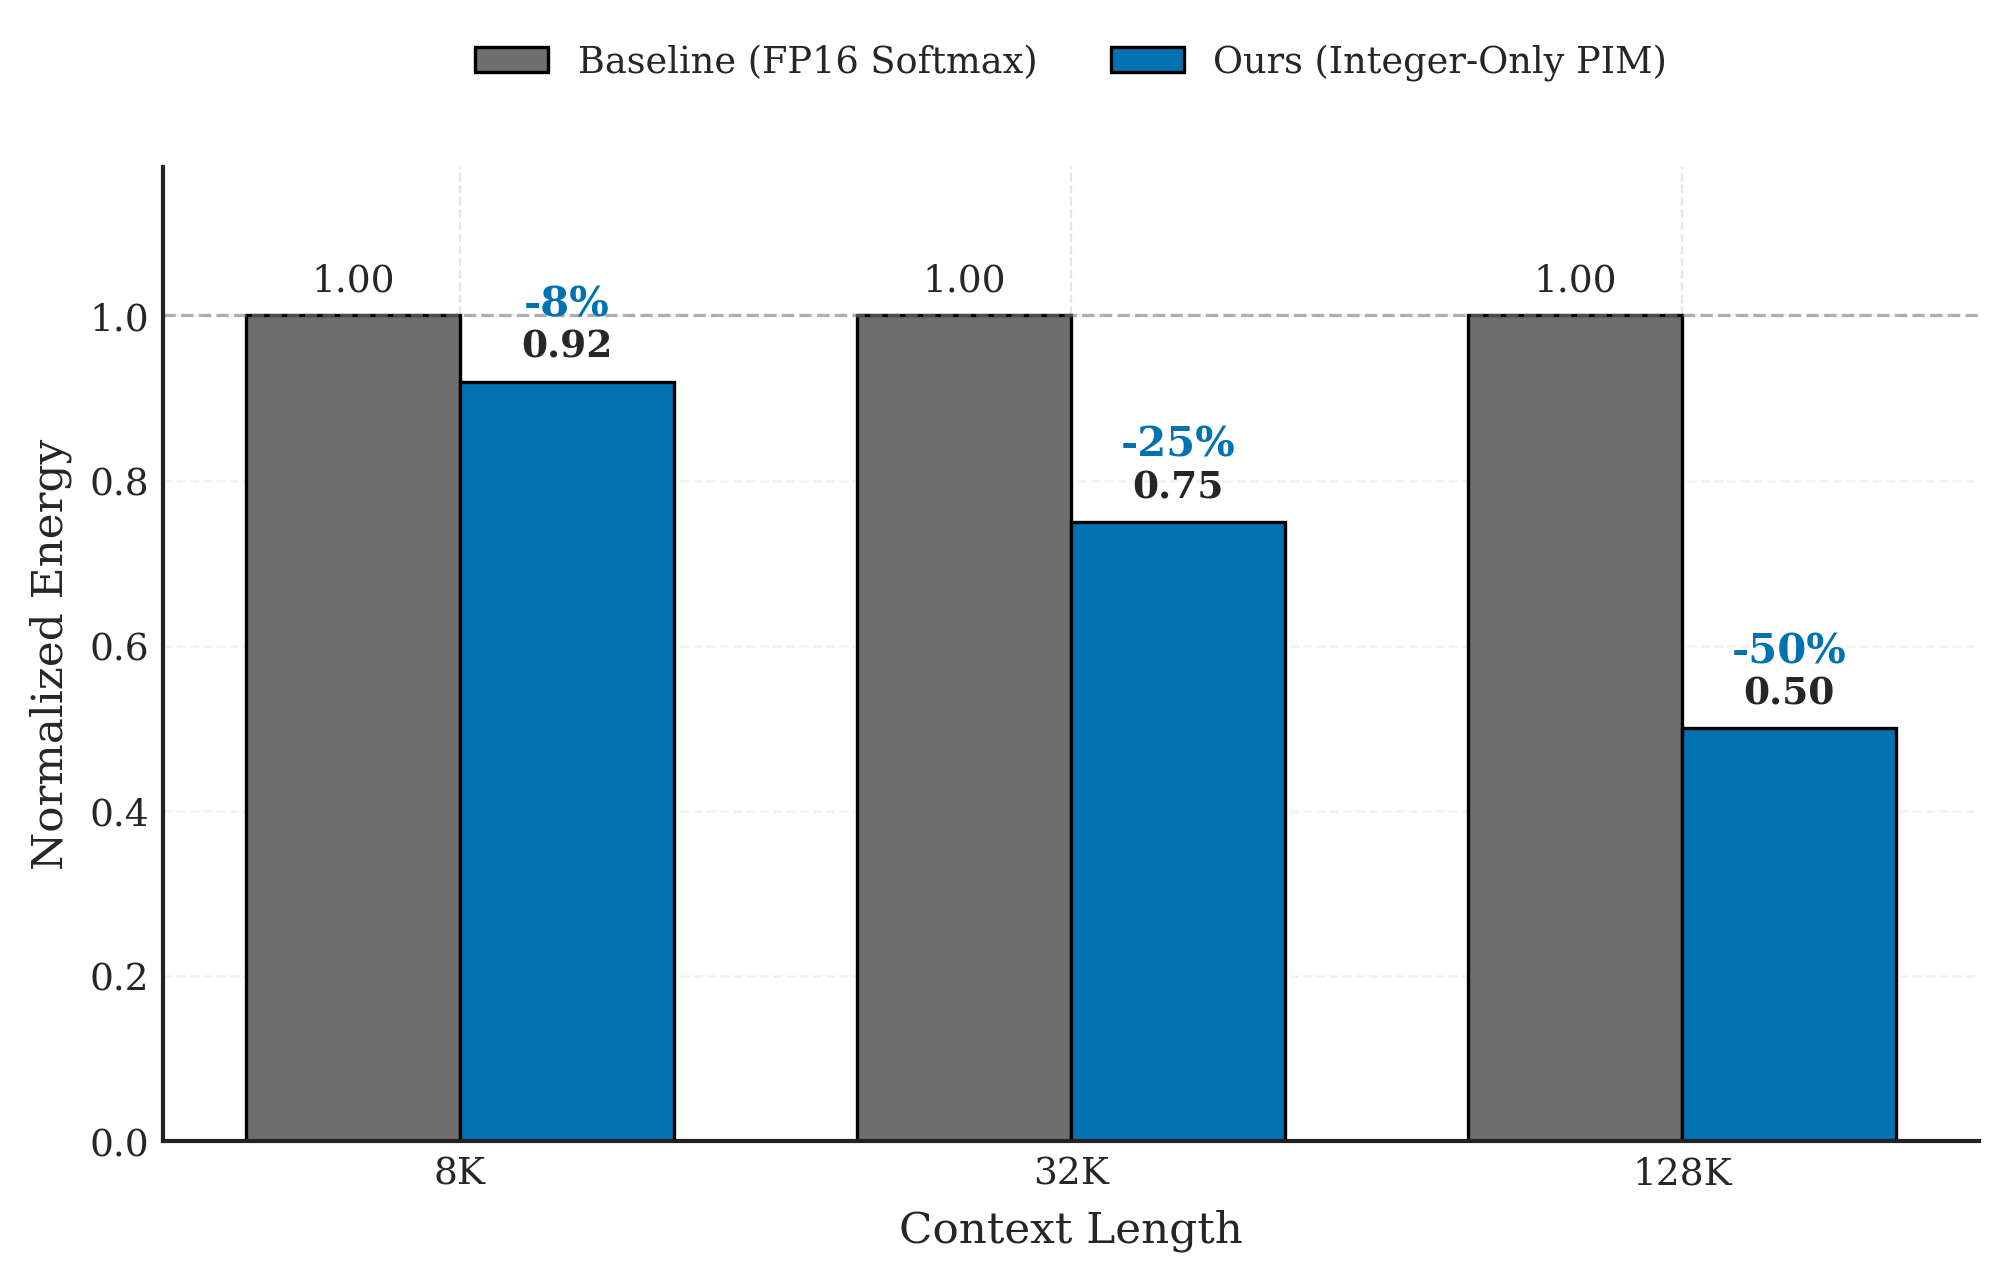
\includegraphics[width=0.78\textwidth]{../paper_assets/figures/fig2_energy_comparison.png}
    \caption[Normalized energy by context length]{Normalized energy consumption across representative context lengths.}
    \label{fig:energy}
\end{figure}

Figure~\ref{fig:energy} shows the corresponding energy trend. The measured normalized savings are 8.3\% at 8K, 24.9\% at 32K, and approximately 50.0\% at 128K. The savings increase with context length because the avoided off-package traffic grows with the size of the historical KV cache.

Area and energy move in the same direction for different reasons. Area improves because the floating-point nonlinear path is replaced by a smaller fixed-point approximation and a small overflow buffer. Energy improves mainly because the design avoids repeated link traversal of the historical KV state. This distinction matters: the endpoint logic is not free, but in the evaluated setting it is small enough that reduced movement dominates the trade-off.

\section{iNLU Mathematical Fidelity}

\begin{figure}[htbp]
    \centering
    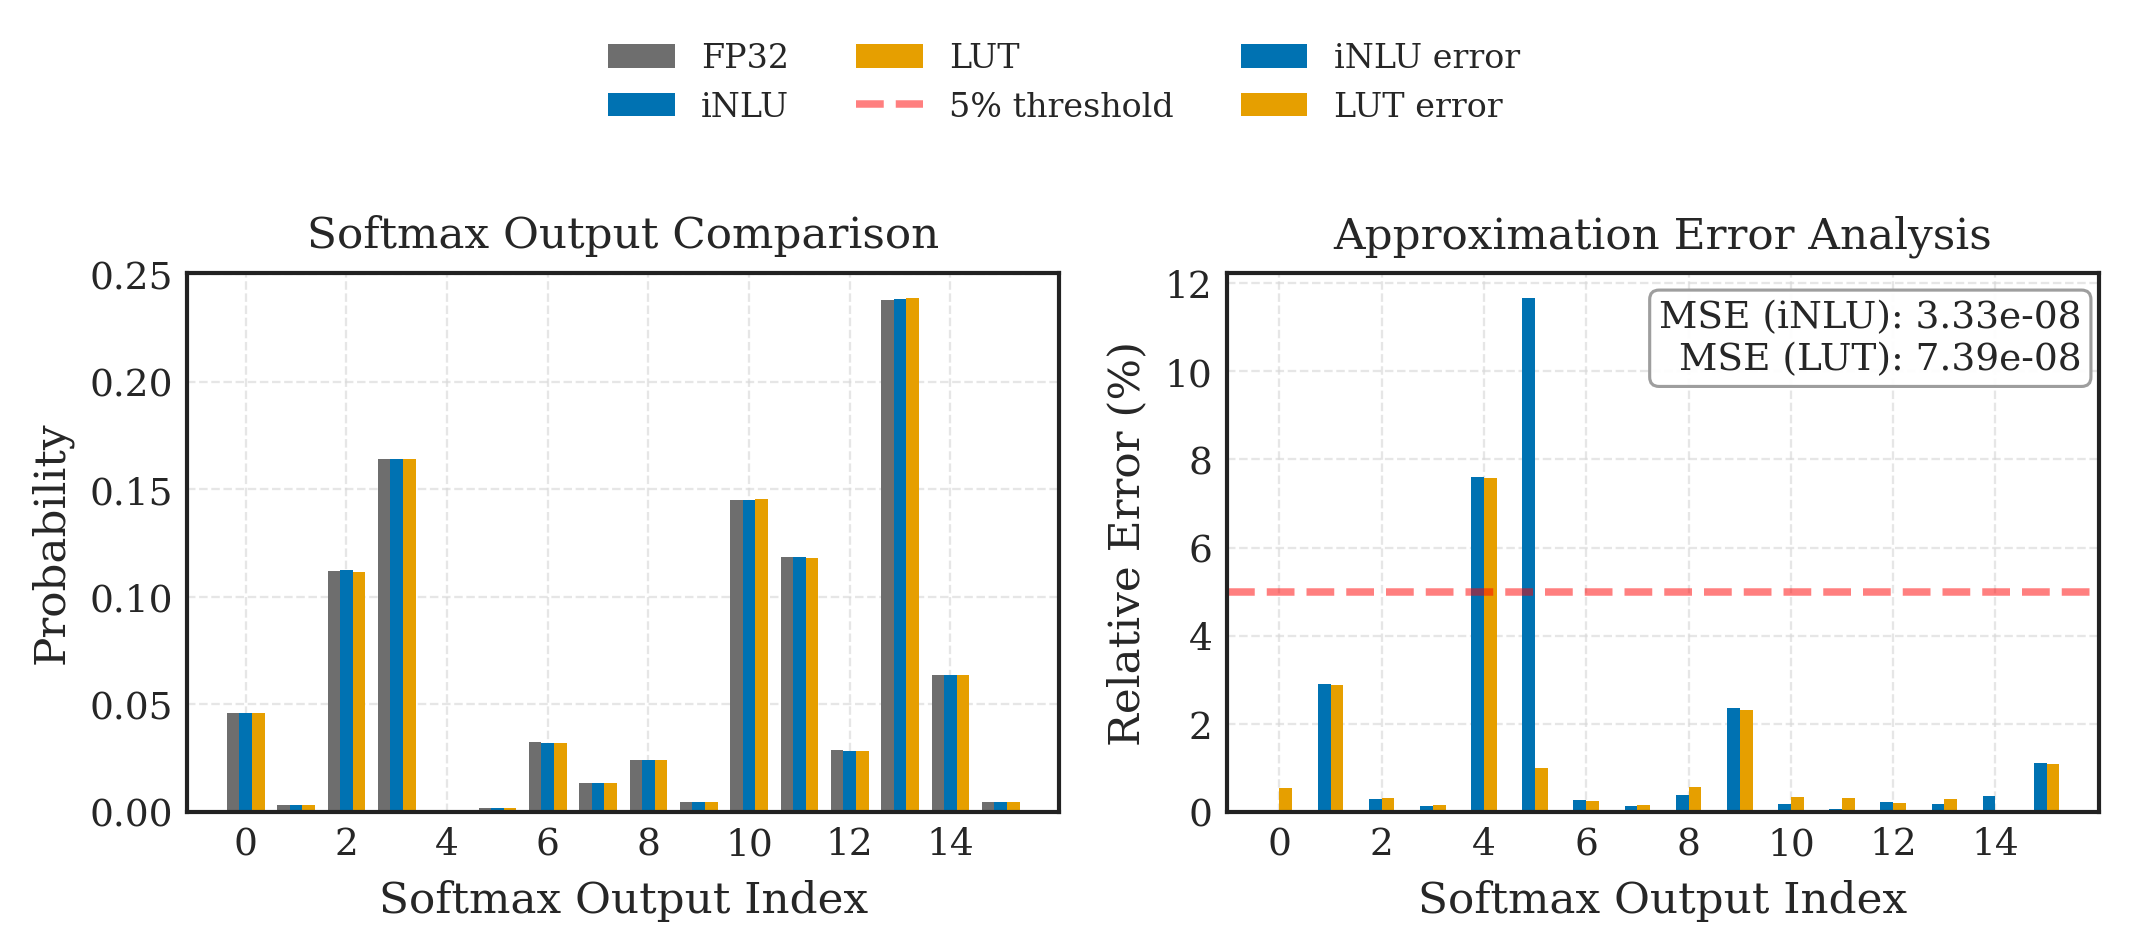
\includegraphics[width=0.9\textwidth]{../paper_assets/figures/fig4_inlu_accuracy.png}
    \caption[iNLU softmax-approximation fidelity]{Softmax output comparison and approximation error for the iNLU polynomial path versus a lookup-table approximation.}
    \label{fig:inlu_acc}
\end{figure}

\begin{figure}[htbp]
    \centering
    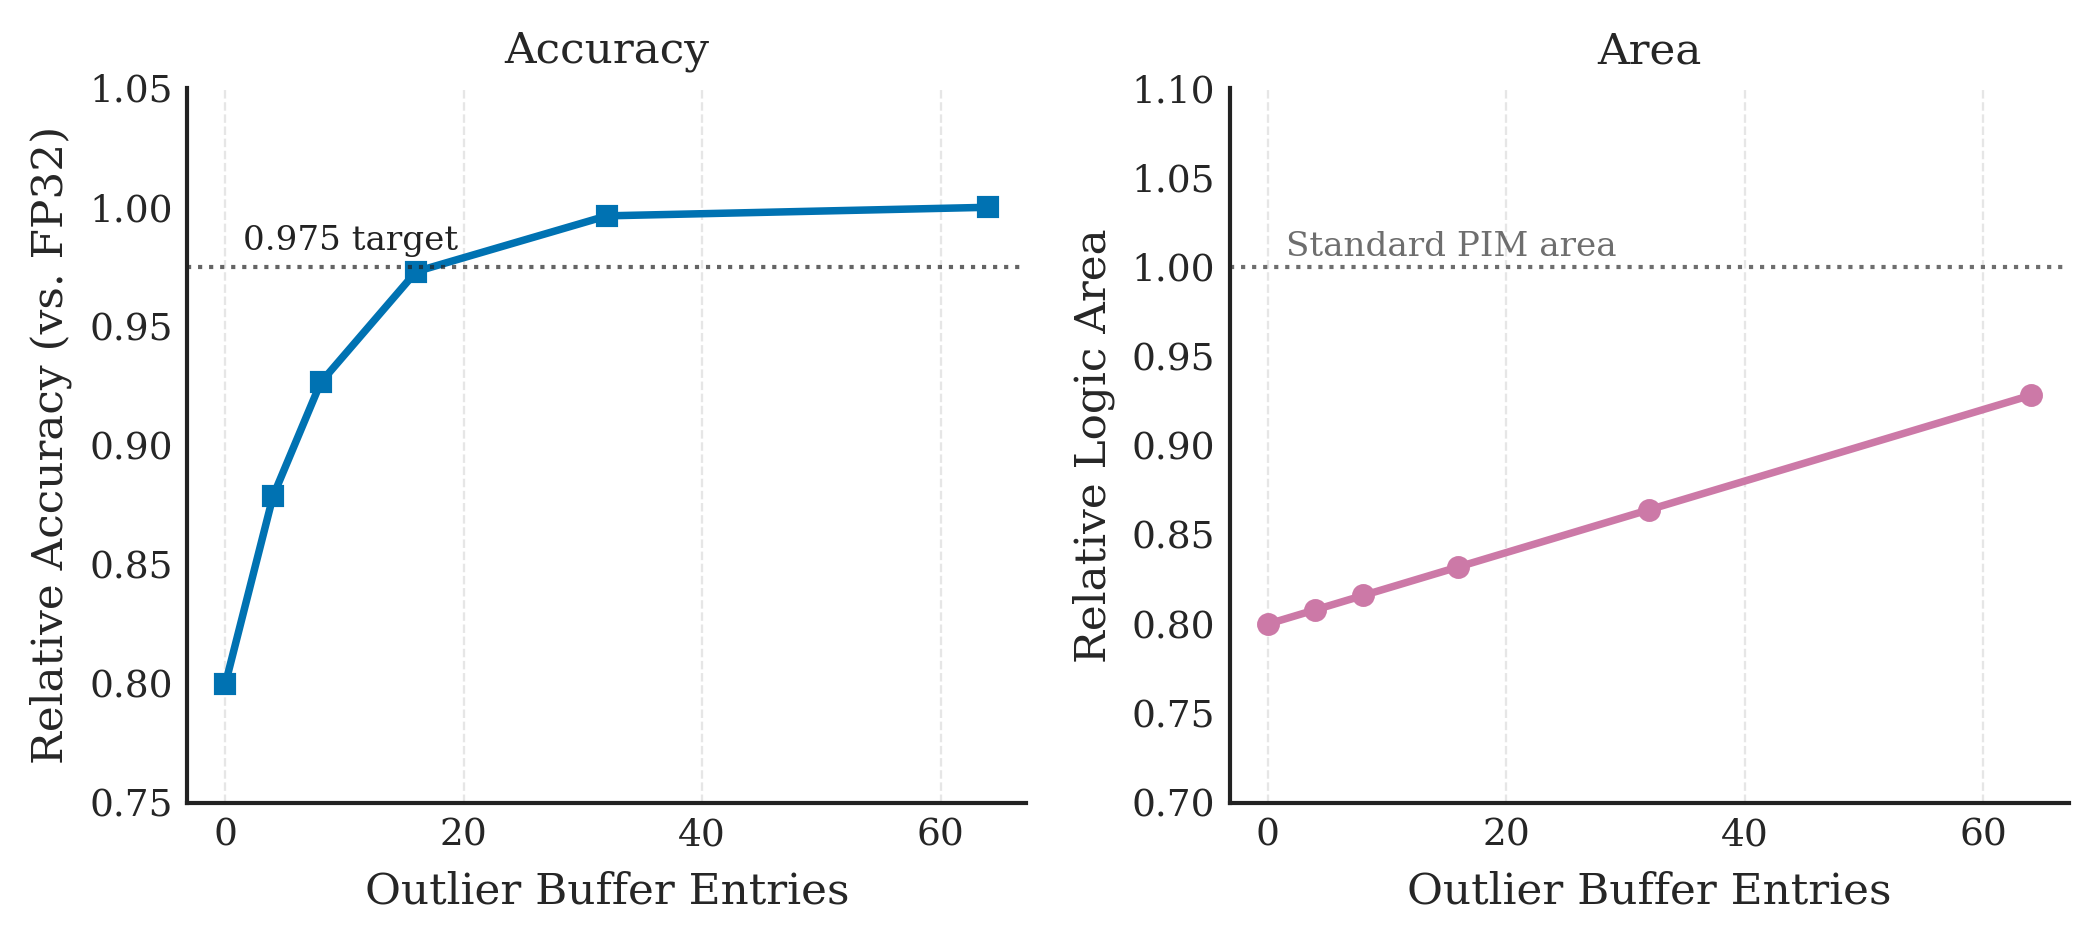
\includegraphics[width=0.9\textwidth]{../paper_assets/figures/fig10_sensitivity_outliers.png}
    \caption[Outlier-buffer sensitivity]{Sensitivity of relative accuracy and relative area to the size of the outlier buffer.}
    \label{fig:sens_outliers}
\end{figure}

\begin{figure}[htbp]
    \centering
    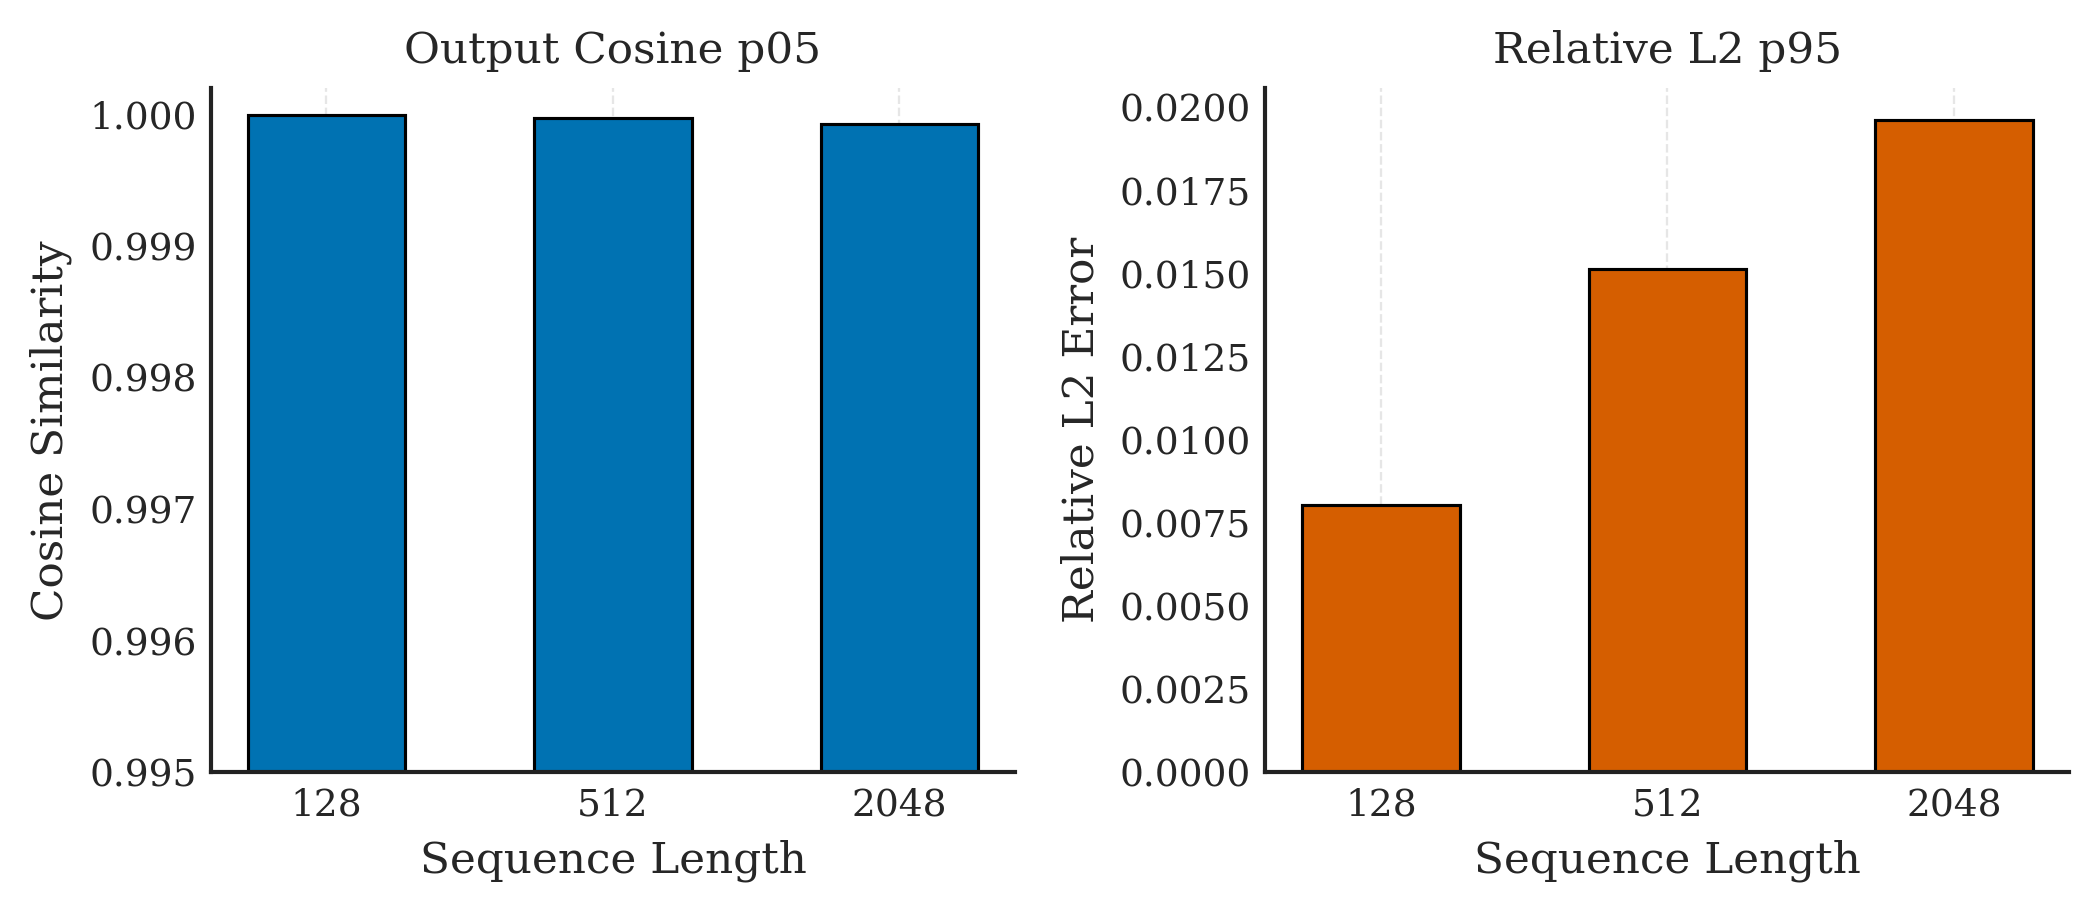
\includegraphics[width=0.78\textwidth]{../paper_assets/figures/fig11_attention_quality.png}
    \caption[Attention-output quality under fixed-point iNLU]{Attention-output quality of the fixed-point iNLU path across sequence lengths.}
    \label{fig:attention_quality}
\end{figure}

Figure~\ref{fig:inlu_acc} checks whether the integer approximation is accurate enough for attention normalization. The plotted iNLU path uses the fixed-point golden model with Q10 logits, the integer polynomial exponential, and Q24 integer normalization. It tracks the FP32 reference closely and has lower mean-squared error than the 64-entry lookup-table alternative in the same figure, about $3.33\times10^{-8}$ versus $7.39\times10^{-8}$. This matters because it addresses the most direct objection to iNLU: the area reduction is not coming from an obviously coarse exponential approximation.

Figure~\ref{fig:attention_quality} moves the check from softmax error to attention behavior. I ran the same fixed-point path in a lightweight single-head Q/K/V attention benchmark over 128, 512, and 2048-token sequences. Across 128 trials per sequence length, the worst 5th-percentile output-vector cosine similarity stays above 0.99992, and the worst 95th-percentile relative $\ell_2$ output error is 1.96\%. This is not a substitute for full language-model perplexity evaluation, but it shows that the integer normalization error remains small at the attention-output level.

Figure~\ref{fig:sens_outliers} isolates the overflow path. A pure INT8 path starts near 0.80 relative accuracy. Adding a 16-entry buffer raises the result to roughly 0.97 while staying near the relative area of the standard PIM baseline. Larger 32-entry and 64-entry buffers approach full relative accuracy, but the gain beyond 16 entries is smaller than the area cost. I therefore use the 16-entry buffer as the practical operating point in the evaluated design.

\section{Multi-Node Scaling and Throughput}

\begin{figure}[htbp]
    \centering
    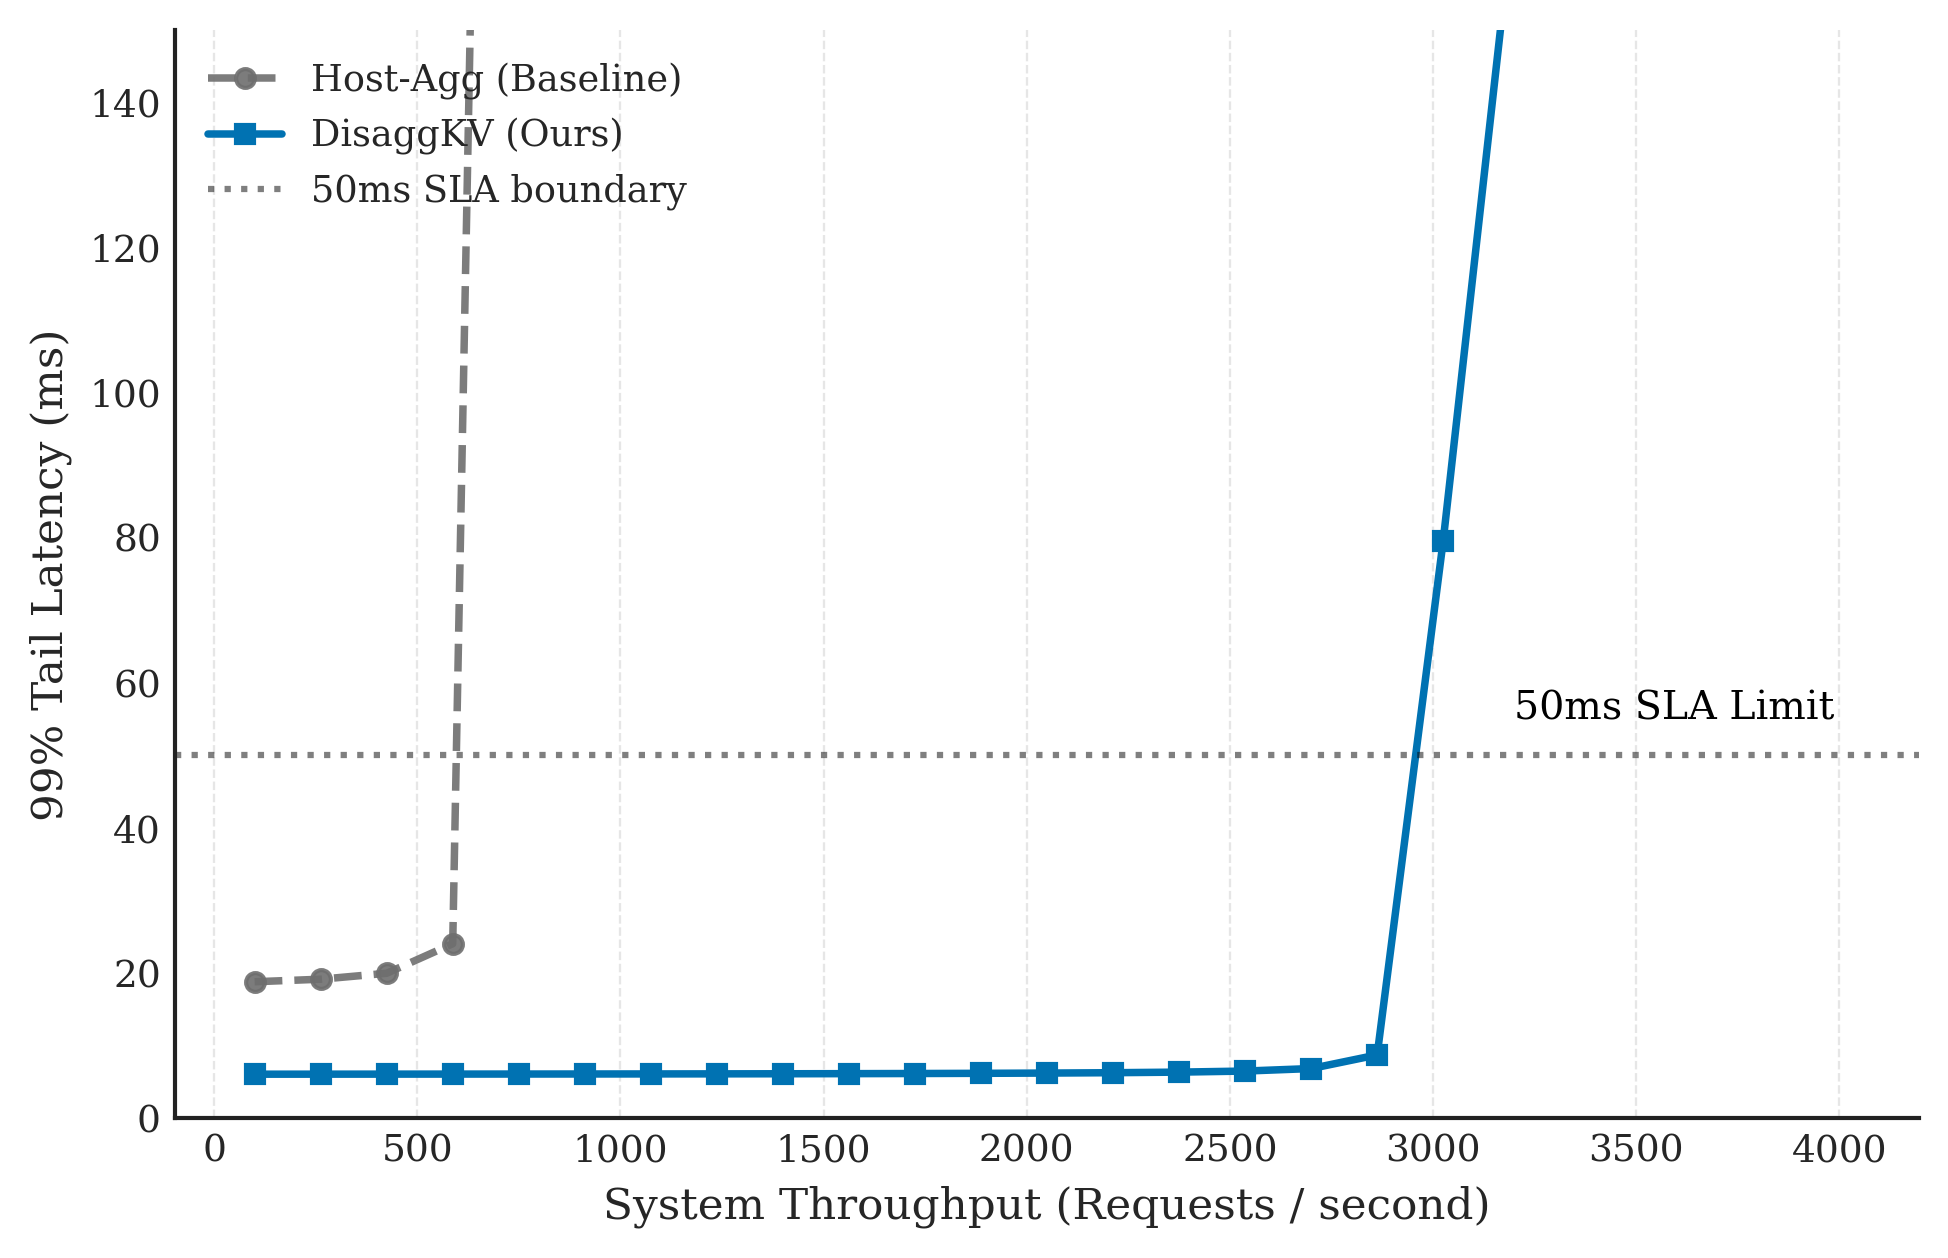
\includegraphics[width=0.82\textwidth]{../paper_assets/figures/fig1_throughput_latency.png}
    \caption[Tail latency versus throughput]{Tail-latency versus throughput for the host-aggregated baseline and DisaggKV.}
    \label{fig:throughput}
\end{figure}

Figure~\ref{fig:throughput} compares modeled throughput and 99th-percentile tail latency using the calibrated queueing model from Chapter~\ref{ch:methodology}. The host-aggregated baseline crosses the 50\,ms SLA boundary slightly above 600 requests/s. DisaggKV remains below 10\,ms through 2.7K requests/s and stays below the 50\,ms target until just under 3.0K requests/s. I compare the designs at the SLA crossing point rather than at the highest plotted point, because that is closer to the operating region a serving system would choose. On that basis, DisaggKV gives roughly a $4.5\times$ throughput improvement over the baseline.

\begin{figure}[htbp]
    \centering
    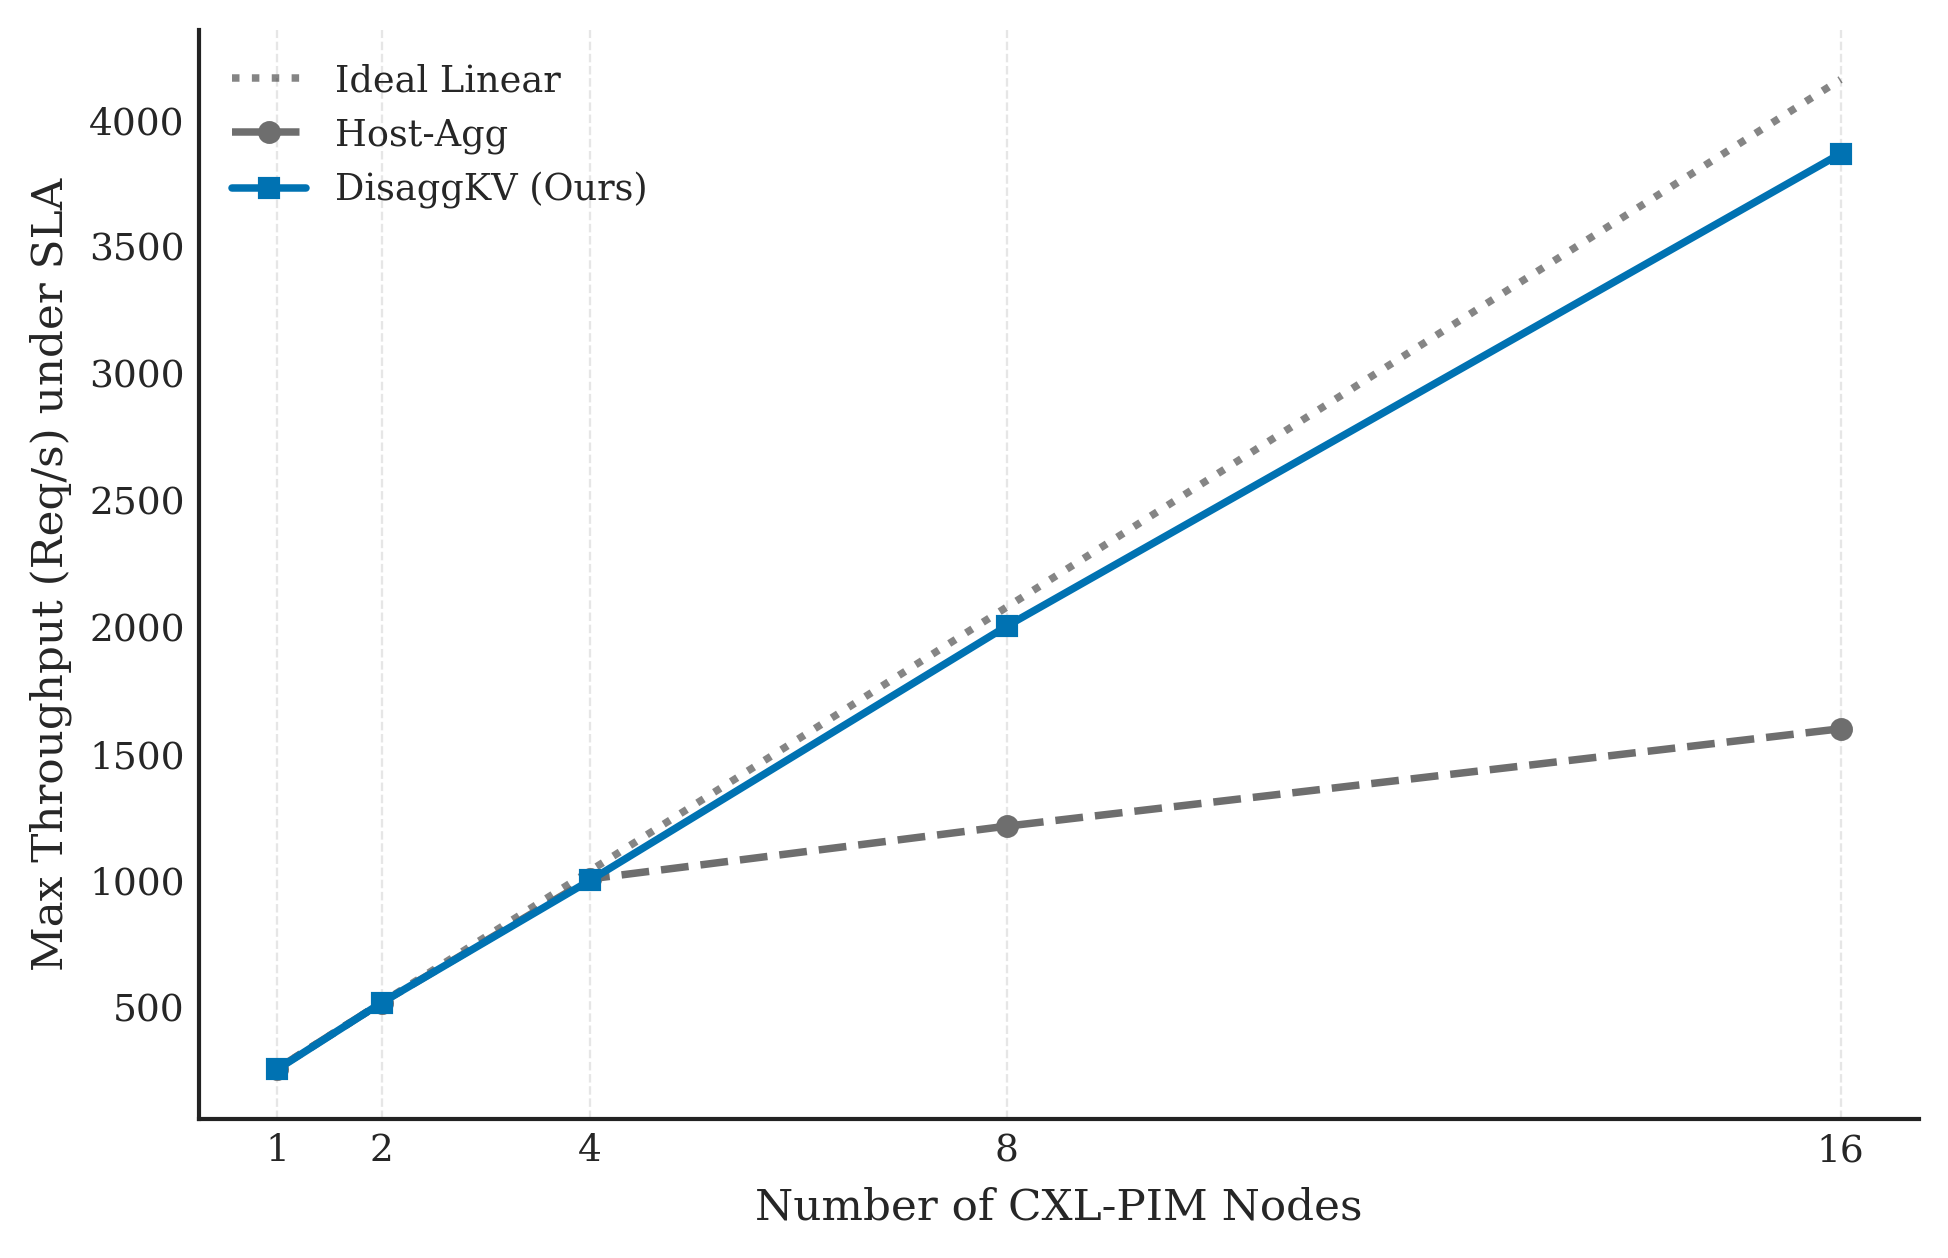
\includegraphics[width=0.82\textwidth]{../paper_assets/figures/fig2_scalability.png}
    \caption[Distributed scalability]{Endpoint-count sweep for DisaggKV in the checked CXL fabric model.}
    \label{fig:scalability}
\end{figure}

Figure~\ref{fig:scalability} plots the endpoint-count sweep. One endpoint serves 257.4 requests/s; eight endpoints reach 2004.9 requests/s, or $7.79\times$ higher throughput. With sixteen endpoints the run reaches 3867.7 requests/s. The useful detail is the change after eight endpoints: capacity and HBM service keep increasing, but reduction barriers start to pull the curve away from an ideal line.

Synchronization explains the bend after eight endpoints. Each added node participates in the two softmax barriers described in Chapter~\ref{ch:disaggkv_system}. DisaggKV keeps those barriers small by exchanging scalars instead of tensors, but it still has to wait for them. The scaling curve is therefore close to linear through eight nodes and visibly below the ideal line at sixteen.

\section{Traffic Accounting and Local Recovery}

\begin{figure}[htbp]
    \centering
    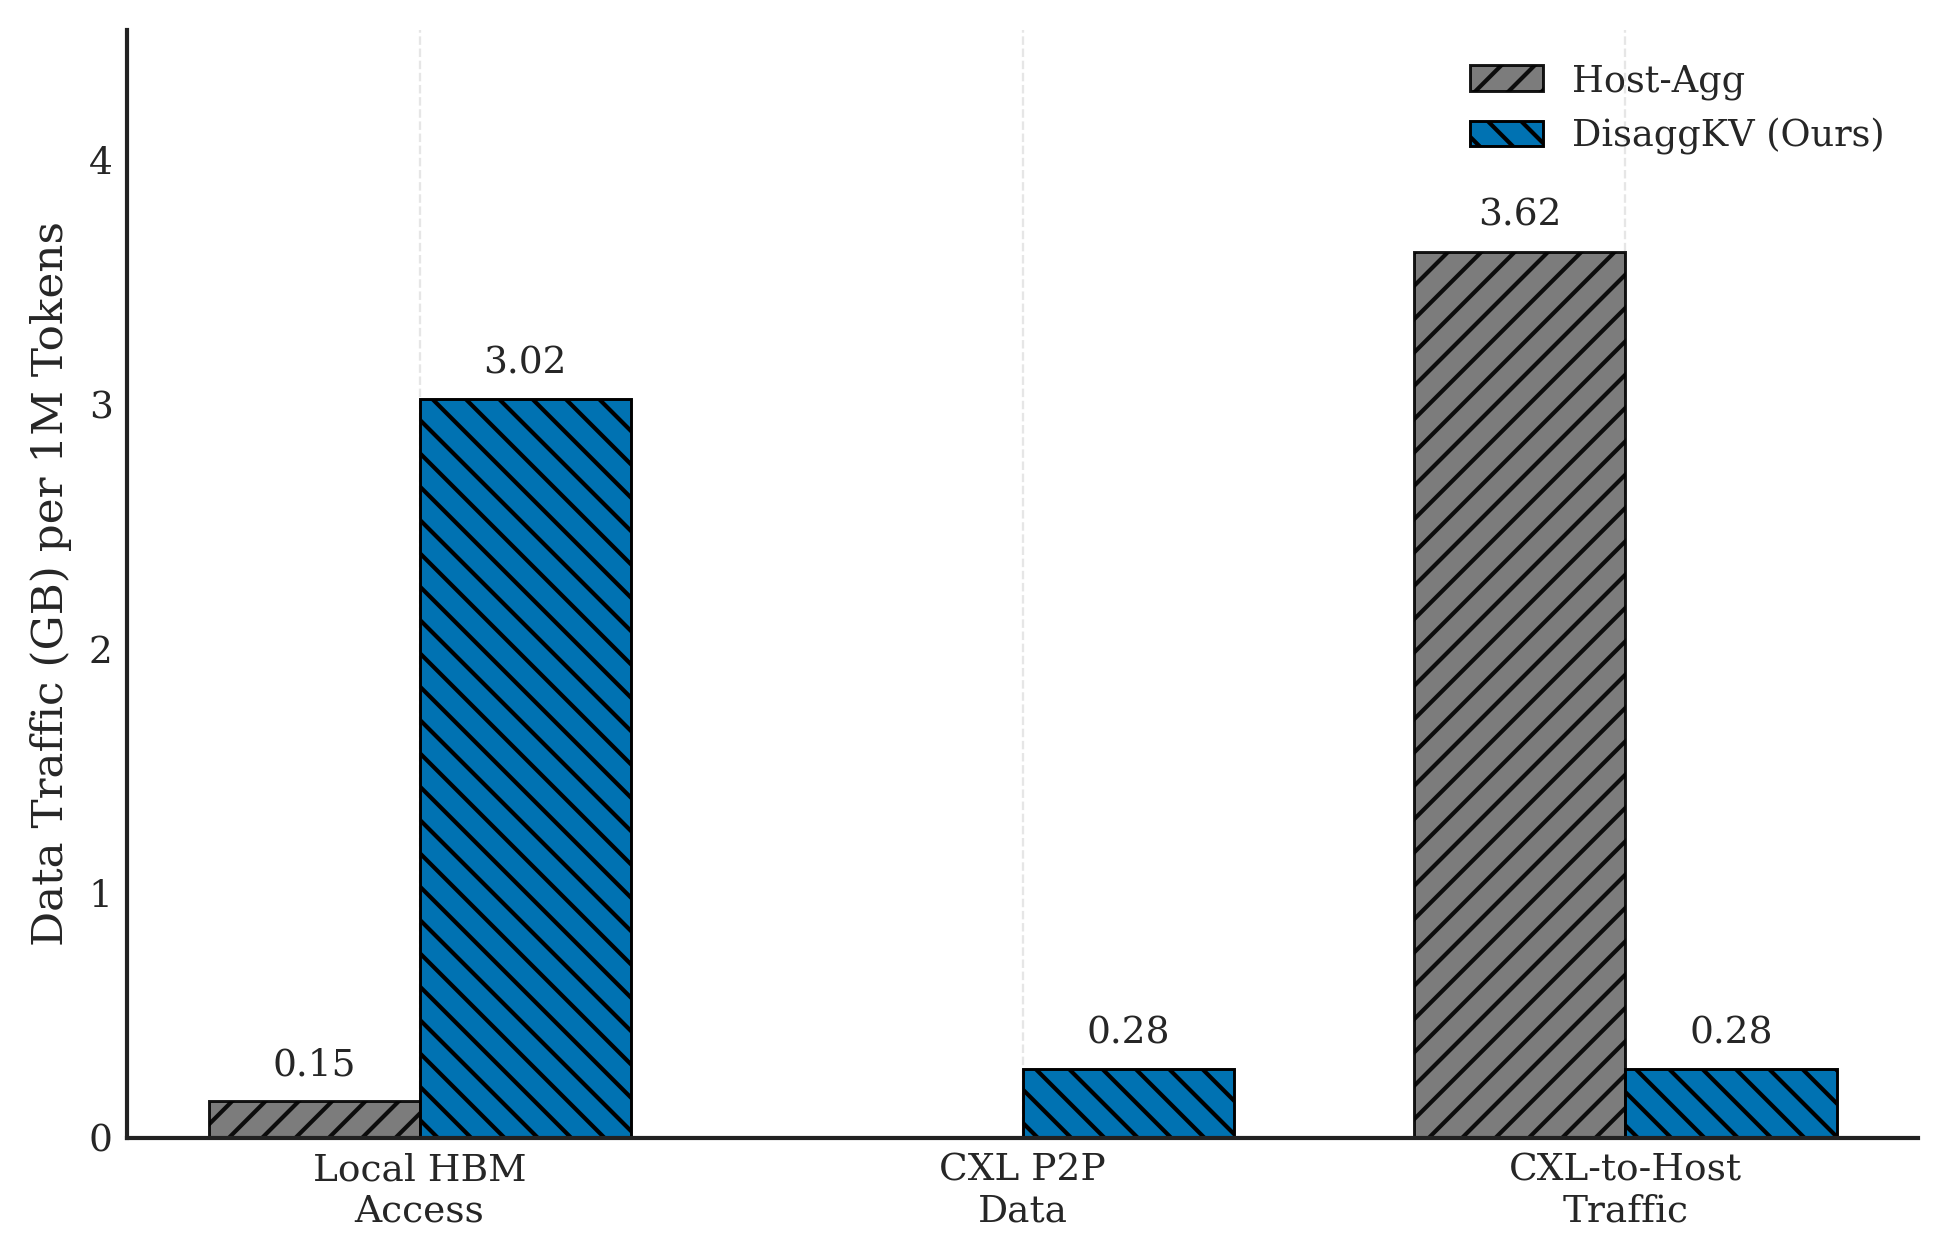
\includegraphics[width=0.82\textwidth]{../paper_assets/figures/fig3_network_breakdown.png}
    \caption[Interconnect traffic breakdown]{Local-HBM, peer-to-peer, and host-facing bytes per 1M decoded tokens in the CXL artifact.}
    \label{fig:network_break}
\end{figure}

The traffic accounting in Figure~\ref{fig:network_break} explains why the latency curve moves. Local HBM access increases because more of the attention work completes on the memory endpoints. Host-facing CXL traffic, however, falls from 3.624\,GB to 0.282\,GB per 1M tokens, a 92.2\% reduction. Even after peer-to-peer reduction traffic is counted, total interconnect traffic remains about 84.4\% below the host-aggregated baseline. These values come from the checked-in CXL fabric artifact and are normalized by the token count of the 50-request trace.

\begin{figure}[htbp]
    \centering
    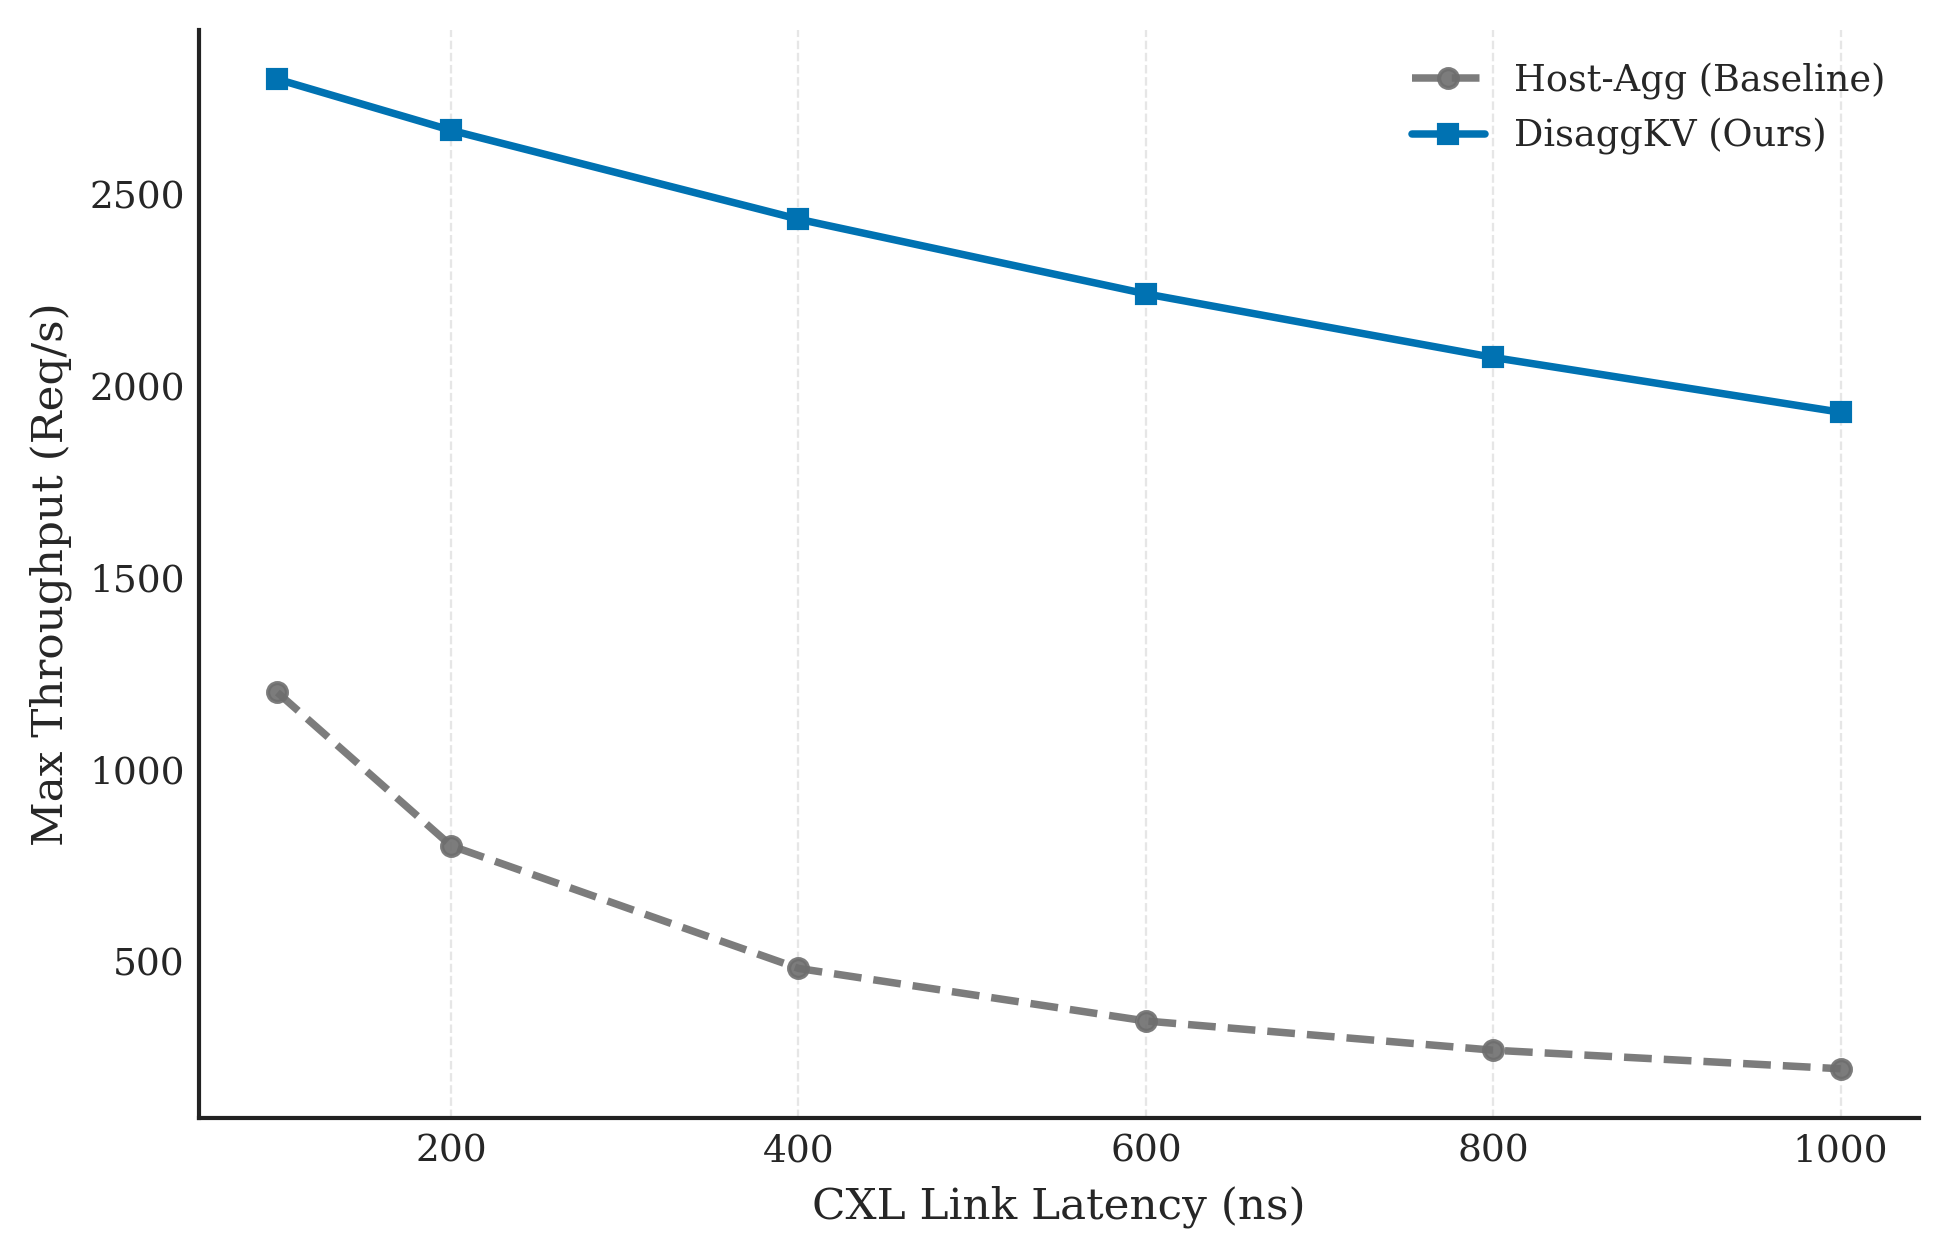
\includegraphics[width=0.82\textwidth]{../paper_assets/figures/fig5_sensitivity_latency.png}
    \caption[Latency-sensitivity study]{Throughput of both designs when modeled CXL-link latency is swept from 100\,ns to 1\,$\mu$s.}
    \label{fig:sens_latency}
\end{figure}

The latency sweep in Figure~\ref{fig:sens_latency} uses the same workload while stretching the CXL-link delay from 100\,ns to 1\,$\mu$s. Under that sweep, the host-aggregated baseline drops from roughly 1200 to 230 requests/s, while DisaggKV drops from roughly 2780 to 1930 requests/s. DisaggKV is not latency-insensitive, since the reduction barriers still cross the fabric. It tolerates the sweep better because its communication pattern is dominated by compact scalar reduction rather than dense tensor fetches.

\begin{figure}[htbp]
\centering
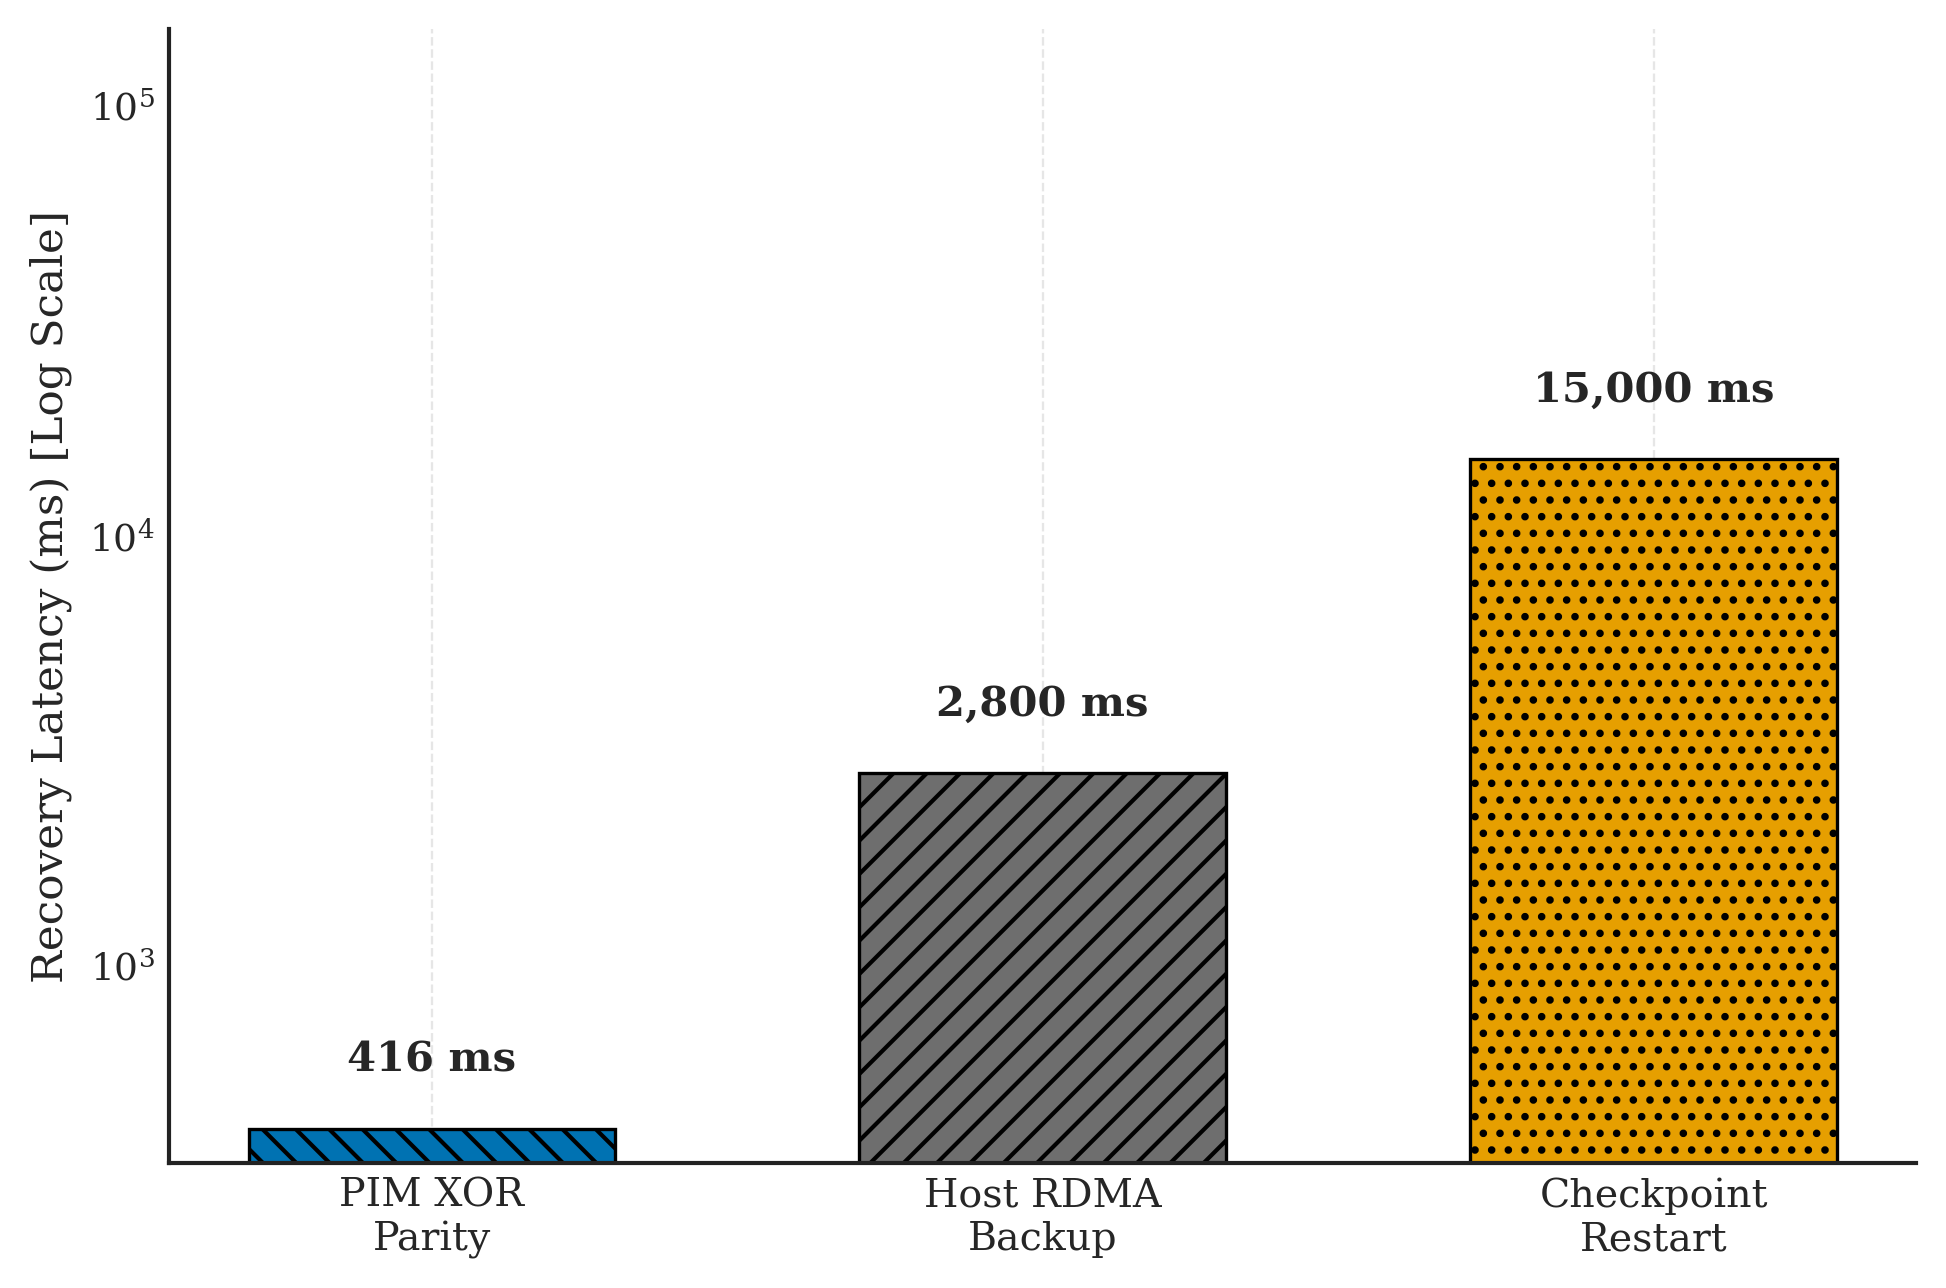
\includegraphics[width=0.78\textwidth]{../paper_assets/figures/fig4_fault_recovery.png}
\caption[Fault-recovery latency comparison]{Recovery-latency distribution for parity-assisted endpoint repair and two host-managed alternatives.}
\label{fig:fault_recovery}
\end{figure}

Figure~\ref{fig:fault_recovery} gives the recovery measurements from the fault-injection artifact. With parity assistance inside DisaggKV, the 95th-percentile recovery time is 416.384\,ms. The two comparison paths are slower by construction: the host-level RDMA backup path is modeled at 2.8\,s, and checkpoint-restart recovery is modeled at 15\,s. The useful point is not only the smaller number; the repair stays close to the endpoint group instead of forcing the host to restart the whole serving path.

The resilience result should be read as localized recovery, not as a complete high-availability design. It shows that short disruption in the endpoint group can be hidden with parity-assisted reconstruction at sub-second timescales in the modeled setting. Persistent device loss, rack-level failures, and request-replay policy require a broader runtime layer than the one evaluated here.

\chapter{Related Systems and Architecture Work}
\label{ch:related_work}

The nearby literature overlaps with this report in vocabulary, but not always in data path. CXL papers usually ask how to expose or place more memory. PIM papers ask which arithmetic can move toward the arrays. Serving-system papers decide how KV pages are scheduled, cached, or reused. Compression papers reduce the number of bytes in the cache. This chapter separates those roles from the narrower point I make here: for long-context decode, the attention traversal and the softmax metadata exchange should move toward the stored KV state.

\section{CXL Work Closest to This Report}

The CXL work closest to this report is mainly concerned with capacity and placement. Pond studies memory pooling for cloud platforms; DirectCXL exposes disaggregated memory through direct access; TPP manages page placement in a CXL-enabled tiered hierarchy~\cite{cxl_pond, direct_cxl, tpp}. CXL-ANNS applies the same broad idea of CXL-backed capacity to memory-intensive approximate-nearest-neighbor search~\cite{cxl_anns}. These systems are important baselines for the memory tier, but they do not move the softmax reduction for a long KV cache into the CXL endpoint.

I separate DisaggKV from page-placement work at the point where the page is already resident. Decode still has to normalize attention over the K/V values stored on that page, and in a pooled system the relevant pages may sit on several endpoints. DisaggKV is aimed at that later step. The fabric carries the scalar coordination payload for softmax instead of serving only as a larger load/store tier for remote memory.

In other words, the remaining question is what happens after the page has been found. If normalization still runs on the host-facing side, long histories continue to move as dense tensors. DisaggKV changes the payload mix: query vectors, scalar reduction state, and compact outputs replace repeated transfers of historical K/V tensors.

\section{Processing-in-Memory for Neural Networks}

PIM is relevant because it attacks the same movement cost from the hardware side. Samsung's HBM-PIM and related accelerator-in-memory designs show that arithmetic can be integrated within or near stacked-memory logic layers~\cite{samsung_pim, aim_samsung}. Transformer-oriented work such as TransPIM and AttentionLego brings that idea closer to attention and sequence workloads~\cite{transpim, attentionlego}.

The difference is not that those PIM systems ignore attention; it is the numerical contract they preserve. Designs that support a broader kernel mix often keep floating-point nonlinear hardware. LKC-CXL-PIM intentionally narrows that contract to quantized attention over resident KV pages. Its iNLU borrows the motivation of integer-only quantization work such as I-BERT, but places the nonlinear approximation beside a near-memory attention engine rather than in a conventional accelerator pipeline~\cite{llm_int8, pim_quant, goliath}.

\section{Serving-Stack Work Above the Fabric}

LLM serving work attacks a different layer of the same pressure. The vLLM system introduced PagedAttention to improve KV-cache management within a single-node serving stack~\cite{vllm}. Orca and FlexGen study scheduling and memory-management strategies for high-throughput autoregressive generation~\cite{orca, flexgen}. DistServe and Splitwise further separate prefill and decode across different compute resources to improve serving efficiency~\cite{distserve, splitwise}.

Distributed-attention work is the closest in spirit because it also splits attention or KV state across devices~\cite{ring_attention, seq_parallel, infinite_llm}. Those systems usually assume GPU memory or accelerator-class collectives. DisaggKV sits lower in the memory hierarchy: a CXL endpoint pool where page locality and scalar endpoint reductions replace part of the host-visible collective path.

\section{KV-Cache Compression and Hierarchical Caching}

Another line of work reduces the amount of KV state that must remain in fast memory. KIVI and KVQuant study low-bit KV-cache quantization and show that careful treatment of key and value distributions can preserve model quality while reducing the cache footprint~\cite{kivi, kvquant}. CacheGen compresses and streams reusable KV caches to reduce context-loading delay across the network~\cite{cachegen}. ShadowKV reduces long-context memory pressure by storing a compact key representation and reconstructing sparse KV pairs on demand~\cite{shadowkv}. Strata studies hierarchical context caching and scheduling for production long-context serving, emphasizing the cost of moving cached contexts back toward the GPU~\cite{strata}.

I view these systems as complementary rather than competing. Compression reduces how many bytes represent the cache. Hierarchical caching improves where those bytes sit and when they are loaded. LKC-CXL-PIM and DisaggKV ask the next data-path question: after the bytes are stored, can decode computation move closer to them? A complete serving stack could combine the directions. Compressed or hierarchically cached KV pages could still be processed by a near-memory endpoint, and endpoint-side reduction could reduce the traffic that remains.

\section{Positioning Summary}

Table~\ref{tab:related_positioning} summarizes this positioning. The central contribution is not a new attention algorithm, a new model architecture, or a general CXL memory manager. It is a hardware-software dataflow for long-context serving that treats the KV cache as the memory-system anchor.

\begin{table}[htbp]
\centering
\caption[Positioning against related work]{Positioning of this report relative to nearby systems and architecture work.}
\label{tab:related_positioning}
\small
\begin{tabularx}{\textwidth}{>{\raggedright\arraybackslash}p{0.22\textwidth}>{\raggedright\arraybackslash}p{0.28\textwidth}>{\raggedright\arraybackslash}X}
\toprule
\textbf{Research Line} & \textbf{Representative Work} & \textbf{Difference from This Report} \\
\midrule
CXL memory pooling & Pond, DirectCXL, TPP & Expands or manages memory capacity, but generally keeps the host-centered load/store data path for remote state. \\
PIM neural kernels & HBM-PIM, AIM, TransPIM, AttentionLego & Moves neural arithmetic near stacked memory; this report specializes the endpoint path for quantized KV-cache softmax instead of a broad floating-point PIM engine. \\
Serving-stack schedulers & vLLM, Orca, FlexGen, DistServe, Splitwise & Improves batching, paging, or prefill/decode placement, while this report changes the memory-endpoint path used when decode revisits old KV pages. \\
Distributed attention & Ring Attention, sequence parallelism, Infinite-LLM & Splits attention across accelerator resources; DisaggKV studies a lower CXL endpoint pool and exchanges scalar softmax state there. \\
KV compression and caching & KIVI, KVQuant, CacheGen, ShadowKV, Strata & Shrinks or reorganizes the cache representation; LKC-CXL-PIM and DisaggKV instead change where the remaining KV attention work runs. \\
\bottomrule
\end{tabularx}
\end{table}

\chapter{Conclusion and Future Work}
\label{ch:conclusion}

This report started from the part of long-context serving that becomes hard to ignore at large context sizes: the KV cache grows with the conversation, and decode returns to that history one token at a time. I studied the problem at two levels, first inside one CXL-attached HBM endpoint and then across a distributed CXL memory pool.

\section{What the Artifacts Show}

The single-node result is mostly a data-movement result. LKC-CXL-PIM is not just extra memory behind the host; it changes where the repeated attention traversal runs. In the evaluated 128K-token case, read latency falls from 77.90 million cycles to 0.80 million cycles, and normalized logic-die area drops from 1.00 to 0.83. The important detail is that locality and numeric format have to move together. Near-memory attention is much less useful if the endpoint first expands the compact cache into a floating-point path.

At pool scale, I would phrase the lesson in terms of coupling. A shared prefix page should remain easy for later requests to attach to; a private continuation page should not quietly turn one endpoint into the request's history store; and the shards still need one maximum and one exponential sum for the current token. In the modeled workload, DisaggKV stays under the 50\,ms tail target until about 2.9K requests/s, scales nearly linearly through eight nodes, and recovers within one second in injected-fault runs. The result is modest, but useful for the design direction: the CXL fabric can carry endpoint-side reduction messages instead of repeatedly pulling much larger historical K/V tensors back through the host-facing path.

\section{Future Outlook}

The next step I would trust most is a prototype that reduces the modeling distance in this report. The current evidence comes from cycle-level memory simulation, event-driven fabric simulation, and synthesis-derived proxy estimates. A fuller RTL or hardware platform would expose controller timing, physical integration cost, and the interaction with a real host runtime. The scheduler also needs experiments with larger fabrics, richer topologies, and workload mixes that change over time. Finally, the iNLU path should be evaluated with end-to-end perplexity and downstream-task measurements, not only the softmax and attention-output checks used here.

The results do not close the topic, but they make the design direction clearer. Long-context serving does not have to stay tied to host-centric KV-cache movement. Integer near-memory execution and peer-to-peer CXL reduction provide a practical path for scaling the memory side of long-context LLM systems.


\backmatter
\bibliographystyle{IEEEtran}
\bibliography{references}

\end{document}
